% main_co2_nature_20260826.tex  (Nature-family restructure, 2026-08-26 night)
% Restructured from main_co2_20260826.tex (article version, preserved).
% Format: unreferenced ~180-word abstract; introductory paragraphs without a
% heading; Results with short bold subheads; Discussion; Methods after
% Discussion; numbered references to be added ([TODO cite] markers remain).
% Display items: 10 main (Tables 1-3, Figs 1-7: attributed map, hetero,
% effcurve, SAF, attribution bars, levels map, mismatch map), all INLINE in
% Results at first citation (per Sunbin 08-26); Extended Data keeps ED
% Tables 1-3 + ED Figs 1-4 (temporal, dlngaci, rfquintile, carbonprice).
% ~3,200 words excl. Methods. New figure: CO2_attribution_bars.png
% (16_attribution_bars.py, from _attribution_scc.csv).
% 08-26 night2 (this copy): SCC valuation added = abstract clause, SCC
% sentences in the attribution results subsection, valuation method
% sentences in 'Attribution and fuel-switching scenarios [Ray and Lisa]',
% SCC country table tab:scc promoted to the Results body (after the
% attributed map; data _attribution_scc.csv via 14_attribution_scc.py).
% NOTE: CO2_map_attributed_2023.png was rebuilt on 08-26 from the Feyrer
% series (15_remake_attributed_map.py) - use the updated PNG on Overleaf.
% Target journal not yet fixed (Nature Sustainability / Nature Communications
% both fit this format); adjust lengths at submission.
\documentclass[12pt]{article}
\usepackage[margin=2.2cm]{geometry}
\usepackage{amsmath,graphicx,booktabs,threeparttable,float}
\title{How Much Does Air Connectivity Increase Aviation CO$_2$?}
\author{[author order TBD]}
\date{Nature-format draft, 26 August 2026}
\begin{document}
\maketitle

\begin{abstract}
\noindent Air connectivity is an explicit object of national policy, yet its
carbon consequences have never been estimated causally at the global level.
Here we construct flight-stage-resolved CO$_2$ for more than 6{,}000
airports over 1996--2023 from schedule data, match it to a global panel of
airport connectivity, and identify the effect of connectivity on emissions
with an instrument based on each country's air-versus-sea market-access
geography. A one percent increase in connectivity raises national aviation
CO$_2$ by 5.7 percent, an elasticity far above one and invariant to how
emissions are allocated across countries. Connectivity growth lowers
emissions per seat-kilometre, but this efficiency margin offsets less than
one tenth of the traffic response. The elasticity is concentrated in
low-income, newly connecting countries, and emissions respond strongly to
neighbouring countries' connectivity through larger aircraft and a more
international traffic mix. Connectivity growth since 1996 accounts for 42.5
percent (356 Mt) of 2023 aviation CO$_2$, an annual external cost of \$18
billion to \$68 billion at standard social-cost-of-carbon values, and
scenario calculations show that only sustained fuel switching, not the
efficiency gains of network development, materially lowers this level.
\end{abstract}

%=======================================================================
\section*{Main [Yifu]}
%=======================================================================
Air connectivity is an explicit object of national policy. Governments
subsidise routes, expand airport capacity, and negotiate air-service
agreements on the premise that connections to the global air network raise
trade, tourism, and productivity, and a large literature documents such
gains [TODO cite]. Aviation is also among the most difficult transport
sectors to decarbonise: it has no near-term electrification path, and its
emissions are governed by separate international accounting conventions
rather than by national inventories [TODO cite]. The carbon consequences of
connectivity policy are therefore a first-order question, and one for
which, to our knowledge, no causal estimate exists at the global level.

The direction of the effect is not in serious doubt: more connections mean
more flying. The empirical questions concern magnitude and structure.
First, proportionality: does a one percent gain in connectivity raise
emissions by more or less than one percent? Network development changes not
only the amount of flying but its organisation, since hub formation can
consolidate traffic into fewer, fuller, and more efficient movements.
Second, incidence: which countries' emissions respond, and does the
response spill across borders through the network? Third, accounting: the
emissions generated by connectivity growth need not be booked where they
are generated, because international aviation is attributed under bunker
conventions rather than territorially [TODO cite].

We answer these questions with two inputs (Methods). The first is a new
emissions panel: flight-stage-resolved CO$_2$ computed from OAG schedule
data under the EEA/EMEP Guidebook methodology for more than 6{,}000
airports over 1996--2023, disaggregated by flight stage and by domestic and
international traffic, so that national emissions can be constructed under
any allocation rule without double counting. The second is identification:
we instrument a country's connectivity, measured by the Global Air
Connectivity Index (GACI), with the interaction of world aviation
technology and the country's air-versus-sea market-access geography in
1996, in the spirit of Feyrer [TODO cite]. The instrument is strong
(first-stage Kleibergen--Paap $F = 154$) and survives a stress test that
interacts the global cycle with baseline population, income, and airport
capacity, the test that eliminates the alternative instruments we examined
(Methods).

%=======================================================================
\section*{Results [Sunbin]}
%=======================================================================
\subsection*{The emissions elasticity of connectivity is far above one}
Table~\ref{tab:main} reports the central result. Because the question is
whether connectivity growth raises emissions more or less than
proportionally, the relevant benchmark is an elasticity of one. The
two-stage least squares estimate is far above it: a one percent increase in
connectivity raises total bunker CO$_2$ by 5.67 percent (s.e.\ 0.41), and
the hypothesis that the elasticity equals one is rejected at any
conventional level. The estimate is insensitive to how emissions are
assigned to countries, ranging from 5.62 under a 50/50 split of cruise
emissions to 5.92 under the territorial rule, and it is stable across
aggregations of airport connectivity to the country level
(Table~\ref{tab:main}, Panels C--E). Ordinary least squares estimates are
roughly forty percent smaller, consistent with attenuation from measurement
error in the connectivity index. The identifying variation is present in
both halves of the sample once crisis years are set aside. Splitting at the
sample midpoint and excluding the global financial crisis (2008--2009) and
the COVID-19 collapse (2020--2021), the first stage is strong in both
subperiods (Kleibergen--Paap $F$ of 75.0 and 36.7): the elasticity is 5.61
(s.e.\ 0.66) for 1996--2007 and 3.01 (s.e.\ 0.64) for 2010--2023, so the
elasticity declines by roughly half between the network-expansion era and
the mature-network era ($p = 0.005$) but remains far above one in both. The
COVID years alone account for the weak later-period first stage in the
unrestricted split (the first-stage $F$ falls to 7.0 when 2020--2021 are
included), and the efficiency response emerges only in the later period,
with the intensity elasticity moving from $+0.78$ (s.e.\ 0.25) to $-0.98$
(s.e.\ 0.25) (Extended Data Table~\ref{tab:temporal} and Extended Data
Fig.~\ref{fig:temporal}).

The same variation raises seat-kilometres by 6.07 percent, faster than
emissions, so emissions per seat-km fall by 0.40 percent
(Table~\ref{tab:main}, column 6). An efficiency margin therefore exists,
but it offsets less than one tenth of the scale response: the emissions
consequence of connectivity growth is dominated by the volume of additional
flying, not by changes in how efficiently it is produced.

\begin{table}[htbp]
\centering
\begin{threeparttable}
\caption{Air connectivity and aviation CO$_2$: main results}
\label{tab:main}
\footnotesize
\begin{tabular}{lcccccc}
\toprule
 & \multicolumn{1}{c}{Bunker CO$_2$} & \multicolumn{1}{c}{LTO CO$_2$} & \multicolumn{1}{c}{50/50 CO$_2$} & \multicolumn{1}{c}{Intl.\ CO$_2$} & \multicolumn{1}{c}{Seat-km} & \multicolumn{1}{c}{Intensity} \\
 & (1) & (2) & (3) & (4) & (5) & (6) \\
\midrule
\multicolumn{7}{l}{\textit{Panel A. OLS}} \\
  ln GACI (cwm) & 3.585$^{***}$ & 3.043$^{***}$ & 3.566$^{***}$ & 3.874$^{***}$ & 3.941$^{***}$ & -0.355$^{***}$ \\
   & (0.175) & (0.177) & (0.175) & (0.198) & (0.183) & (0.043) \\
  $N$ & 4,634 & 4,634 & 4,634 & 4,633 & 4,634 & 4,634 \\
\midrule
\multicolumn{7}{l}{\textit{Panel B. 2SLS, Feyrer instrument, capacity-weighted mean}} \\
  ln GACI (cwm) & 5.669$^{***}$ & 5.921$^{***}$ & 5.620$^{***}$ & 5.690$^{***}$ & 6.068$^{***}$ & -0.399$^{***}$ \\
   & (0.412) & (0.448) & (0.409) & (0.415) & (0.443) & (0.118) \\
  KP $F$ & 153.6 & 153.6 & 153.6 & 152.7 & 153.6 & 153.6 \\
  $N$ & 4,634 & 4,634 & 4,634 & 4,633 & 4,634 & 4,634 \\
\midrule
\multicolumn{7}{l}{\textit{Panel C. 2SLS, GACI sum}} \\
  ln GACI (sum) & 2.283$^{***}$ & 2.384$^{***}$ & 2.263$^{***}$ & 2.291$^{***}$ & 2.443$^{***}$ & -0.161$^{***}$ \\
   & (0.224) & (0.219) & (0.222) & (0.237) & (0.250) & (0.052) \\
  KP $F$ & 90.3 & 90.3 & 90.3 & 89.5 & 90.3 & 90.3 \\
  $N$ & 4,634 & 4,634 & 4,634 & 4,633 & 4,634 & 4,634 \\
\midrule
\multicolumn{7}{l}{\textit{Panel D. 2SLS, GACI max}} \\
  ln GACI (max) & 4.822$^{***}$ & 5.036$^{***}$ & 4.780$^{***}$ & 4.836$^{***}$ & 5.161$^{***}$ & -0.340$^{***}$ \\
   & (0.329) & (0.348) & (0.327) & (0.343) & (0.361) & (0.101) \\
  KP $F$ & 172.0 & 172.0 & 172.0 & 171.0 & 172.0 & 172.0 \\
  $N$ & 4,634 & 4,634 & 4,634 & 4,633 & 4,634 & 4,634 \\
\midrule
\multicolumn{7}{l}{\textit{Panel E. 2SLS, GACI mean}} \\
  ln GACI (mean) & 5.897$^{***}$ & 6.159$^{***}$ & 5.846$^{***}$ & 5.902$^{***}$ & 6.313$^{***}$ & -0.415$^{***}$ \\
   & (0.591) & (0.623) & (0.587) & (0.593) & (0.624) & (0.122) \\
  KP $F$ & 136.2 & 136.2 & 136.2 & 135.6 & 136.2 & 136.2 \\
  $N$ & 4,634 & 4,634 & 4,634 & 4,633 & 4,634 & 4,634 \\
\bottomrule
\end{tabular}
\begin{tablenotes}[flushleft]
\footnotesize
\item Notes: Country-year panel, 1996--2023. All specifications include country and year fixed effects and control for log population and log sea market access. Outcomes are in logs: total aviation CO$_2$ under the bunker convention (all cruise plus departure-side LTO assigned to the departure country), landing-and-take-off CO$_2$ only, CO$_2$ with cruise split 50/50 between endpoint countries, bunker CO$_2$ from international flights, scheduled departing seat-kilometres, and CO$_2$ per seat-km. The instrument in Panels B--E interacts world aviation technology with air-versus-sea geography (Feyrer-type). Robust standard errors in parentheses. $^{***}$, $^{**}$, $^{*}$: significance at 1, 5, and 10 percent.
\end{tablenotes}
\end{threeparttable}
\end{table}

\subsection*{The elasticity is concentrated in newly connecting countries}
The world average combines countries entering the network with countries
already saturated. Splitting the sample by 1996 characteristics yields a
monotone and steep gradient (Fig.~\ref{fig:hetero} and Extended Data
Table~\ref{tab:hetero}): the elasticity is 11.43 in the bottom income
tercile, 5.91 in the middle, and an insignificant 0.35 at the top, with the
same pattern by baseline connectivity. Regionally, the elasticity is 8.39
in Africa, 5.42 in Asia--Pacific, and 3.23 in Latin America, while Europe
is a precisely estimated zero (0.24, s.e.\ 0.62). The efficiency margin
follows the same geography: emissions per seat-km fall significantly only
in the bottom income tercile. The headline elasticity therefore describes
the network's extensive margin; for mature networks, connectivity growth is
approximately carbon-neutral at the margin.

\begin{figure}[htbp]
\centering
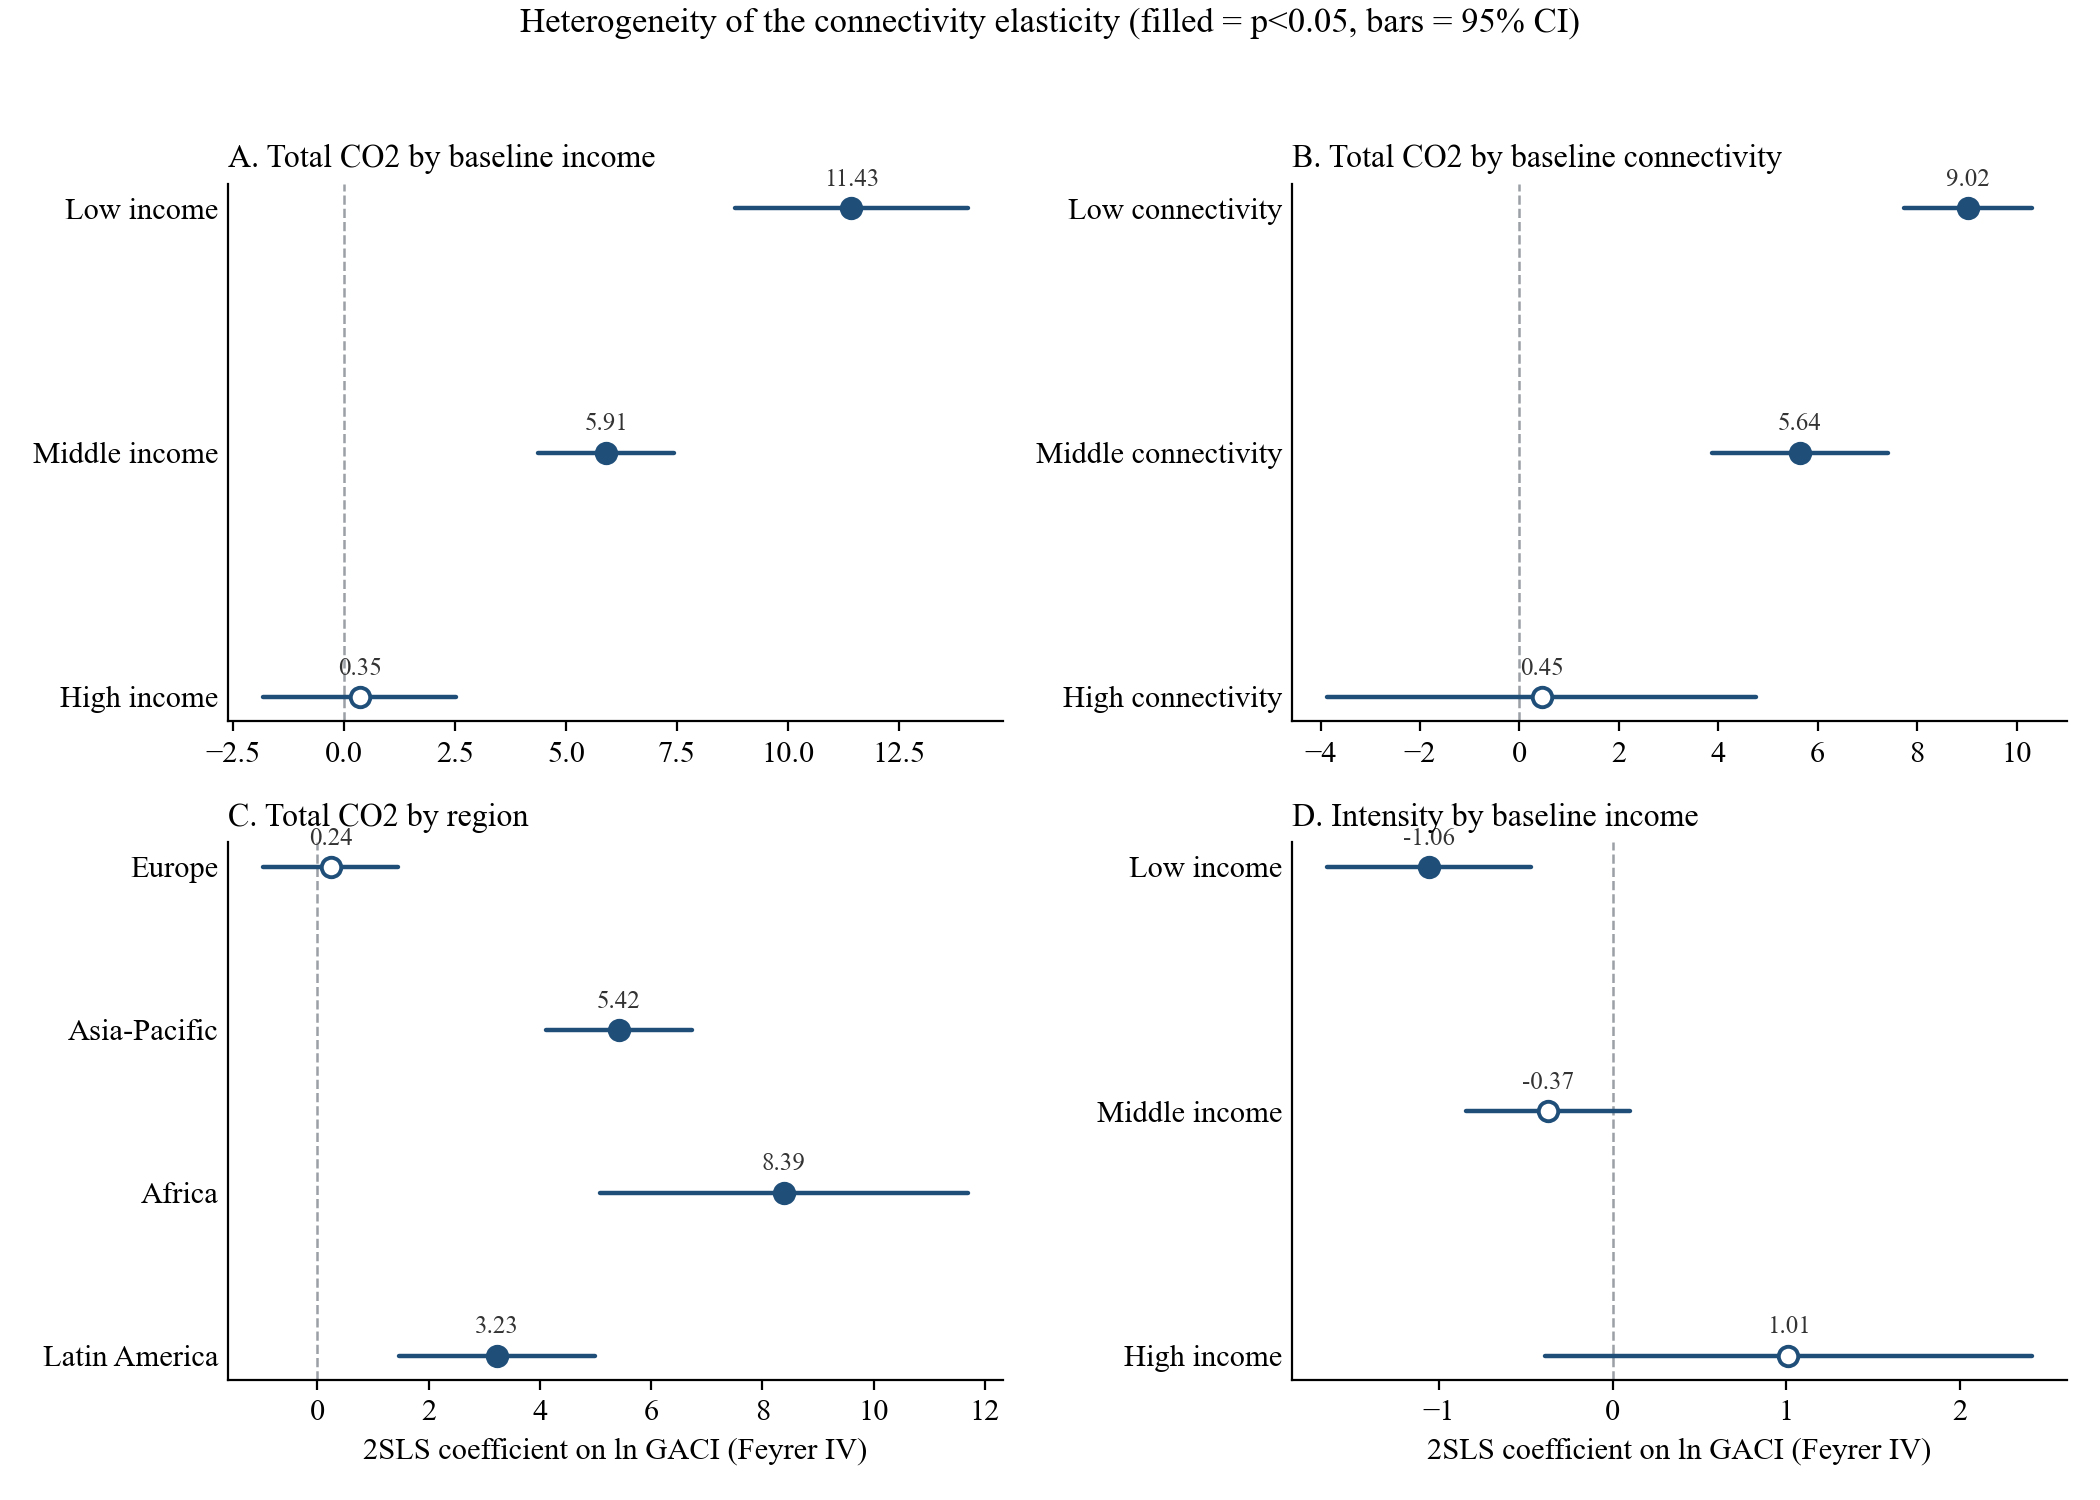
\includegraphics[width=0.92\textwidth]{CO2_hetero_coefplot.png}
\caption{\textbf{Heterogeneity of the connectivity elasticity} (2SLS, Feyrer instrument). Filled markers denote $p<0.05$; bars are 95 percent confidence intervals. The Middle East and North America are omitted as unidentified.}
\label{fig:hetero}
\end{figure}

\subsection*{Traffic volume, not composition, carries the effect}
Causal mediation analysis (Extended Data Table~\ref{tab:mediation})
attributes 86.5 percent of the total effect to seat-kilometres and 83.9
percent to flight frequency, while the international share of traffic
mediates essentially nothing. The connectivity-emissions relationship is
thus a traffic-volume phenomenon. Composition responds to a different kind
of connectivity variation: under a secondary instrument whose compliers are
hub-quality changes rather than market-access growth, total emissions do
not respond but international emissions rise by 3.16 percent and emissions
per seat-km by 1.23 percent, indicating that hub-quality gains recompose
traffic toward international long-haul service rather than scaling it
(Methods).

\subsection*{Emissions respond to neighbouring countries' connectivity}
Emissions do not respond only to a country's own network.
Table~\ref{tab:spillover} instruments the inverse-distance-weighted
connectivity of all other countries with their geography-based shifters,
holding the own shifter fixed. A one percent increase in neighbours'
connectivity raises own bunker CO$_2$ by 7.45 percent (s.e.\ 1.99) and
international CO$_2$ by 10.24 percent, and raises emissions per seat-km.
Trade volume does not respond, so the channel is a change in the structure
of aviation activity rather than trade demand. The margins are the converse
of the own-connectivity response: flight frequency does not move, but
seat-kilometres rise through larger aircraft and a more international
traffic mix, consistent with feeding traffic into foreign hubs. National
estimates therefore understate the network-wide emissions effect of
connectivity growth, and the emissions accrue across borders while the
associated economic gains, as proxied by trade, show no measurable
response.

\begin{table}[htbp]
\centering
\begin{threeparttable}
\caption{Connectivity spillovers: neighbouring countries' connectivity and own aviation outcomes}
\label{tab:spillover}
\footnotesize
\begin{tabular}{lccccc}
\toprule
\multicolumn{6}{l}{\textit{Panel A. 2SLS: neighbour connectivity instrumented}} \\
 & \multicolumn{1}{c}{Bunker CO$_2$} & \multicolumn{1}{c}{Intl.\ CO$_2$} & \multicolumn{1}{c}{Intensity} & \multicolumn{1}{c}{Trade volume} & \\
 & (1) & (2) & (3) & (4) & \\
\midrule
  ln neighbour GACI & 7.454$^{***}$ & 10.237$^{***}$ & 1.312$^{**}$ & 2.072 & \\
   & (1.994) & (2.092) & (0.534) & (2.011) & \\
  Own Feyrer shifter & 0.254$^{**}$ & 0.076 & -0.134$^{***}$ & 0.157 & \\
   & (0.122) & (0.128) & (0.037) & (0.124) & \\
  KP $F$ & 134.1 & 134.0 & 134.1 & 134.1 & \\
  $N$ & 4,623 & 4,622 & 4,623 & 4,623 & \\
\midrule
\multicolumn{6}{l}{\textit{Panel B. Margins of the own response to neighbour connectivity (same specification)}} \\
 & \multicolumn{1}{c}{Flights} & \multicolumn{1}{c}{Seat-km} & \multicolumn{1}{c}{Aircraft size} & \multicolumn{1}{c}{Stage length} & \multicolumn{1}{c}{Intl.\ share} \\
 & (1) & (2) & (3) & (4) & (5) \\
\midrule
  ln neighbour GACI & 2.730 & 6.141$^{***}$ & 5.437$^{***}$ & -2.026$^{**}$ & 1.046$^{***}$ \\
   & (2.216) & (2.083) & (1.170) & (1.008) & (0.281) \\
\bottomrule
\end{tabular}
\begin{tablenotes}[flushleft]
\footnotesize
\item Notes: Neighbour connectivity is the inverse-distance-weighted average of all other countries' log GACI (capacity-weighted mean), with weights based on haversine distances between countries' aviation activity centroids. It is instrumented by the identically weighted average of other countries' Feyrer shifters; the own Feyrer shifter enters directly, so the own-connectivity effect is in reduced form. Own and neighbour connectivity cannot be jointly instrumented because the two shifters are collinear within country. All specifications include country and year fixed effects and control for log population and log sea market access. Robust standard errors in parentheses. $^{***}$, $^{**}$, $^{*}$: significance at 1, 5, and 10 percent.
\end{tablenotes}
\end{threeparttable}
\end{table}

\subsection*{Efficiency improves with connectivity but cannot offset scale}
The country-level intensity decline has a within-country counterpart. In an
airport panel with airport and country-by-year fixed effects, a one percent
increase in an airport's connectivity is associated with a 0.49 percent
decline in CO$_2$ per seat-km and a 0.33 percentage point higher
international share of seat-kilometres (Methods; these estimates are
descriptive, as no valid airport-level instrument is available). The
cross-section is summarised by the efficiency curve in
Fig.~\ref{fig:effcurve}: median intensity falls monotonically from 284 to
77 kg per 1{,}000 seat-km across connectivity ventiles, while the
international share rises from one to sixty percent. The efficiency margin
is real at the node, and it is dominated by scale at the aggregate.

\begin{figure}[htbp]
\centering
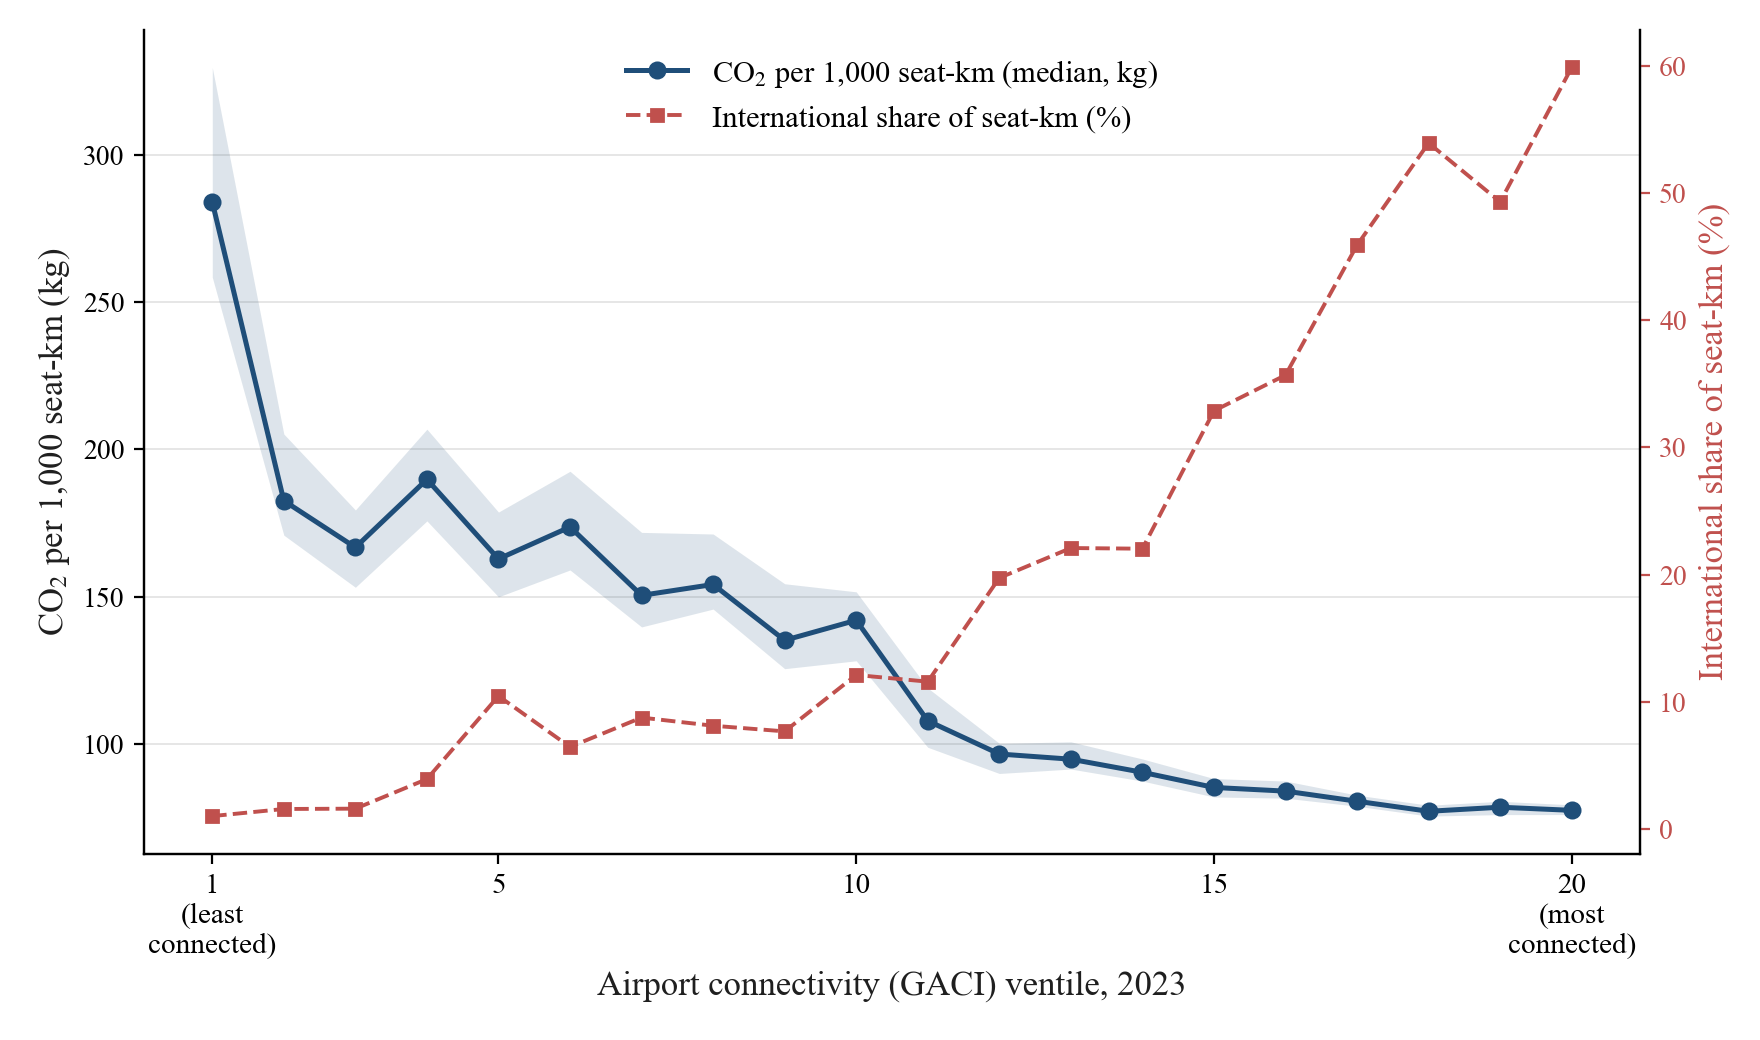
\includegraphics[width=0.92\textwidth]{CO2_efficiency_curve.png}
\caption{\textbf{Airport-level efficiency curve, 2023:} median kg CO$_2$ per 1{,}000 seat-km by connectivity ventile, with the international share of seat-km on the second panel.}
\label{fig:effcurve}
\end{figure}

\subsection*{Connectivity growth accounts for 42.5 percent of 2023
emissions}
Applying the estimated elasticity to each country's connectivity change
since 1996 attributes 356 Mt, or 42.5 percent, of 2023 aviation CO$_2$ to
post-1996 network expansion (Fig.~\ref{fig:attributed}; Methods). The
attributed growth is concentrated in emerging hub countries: China
($+88$ Mt), the United States ($+36$), the United Arab Emirates ($+25$),
Japan ($+17$), Turkey ($+17$), India ($+16$), and Korea ($+14$), while
Germany's declining connectivity contributes $-16$ Mt (Table~\ref{tab:scc} and Fig.~\ref{fig:bars}). Valued at standard social-cost-of-carbon estimates,
these emissions represent an annual external cost of \$18.2 billion to
\$67.7 billion, depending on whether the US Interagency Working Group
interim value (\$51 per tonne), the Rennert et al.\ estimate (\$185), or
the US EPA central value (\$190) is applied [TODO cite]; at the EPA value
the cost is \$16.7 billion per year for China, \$6.9 billion for the
United States, and \$4.7 billion for the United Arab Emirates, while
Germany's connectivity decline corresponds to an avoided cost of \$3.0
billion per year. Where these
emissions are generated is, moreover, not where they are booked: the
bunker-attributed share of world emissions exceeds the physical
landing-and-take-off share by 1.4 percentage points for the United States
and the United Arab Emirates, while China's attributed share falls short by
3.5 points, a gap that is positive at every international mega-hub and
negative at large domestically oriented hubs (Figs.~\ref{fig:levels} and \ref{fig:mismatch}). Any scheme that allocates
responsibility by booked emissions, including CORSIA, embeds a transfer
across these accounting boundaries.

\begin{figure}[htbp]
\centering
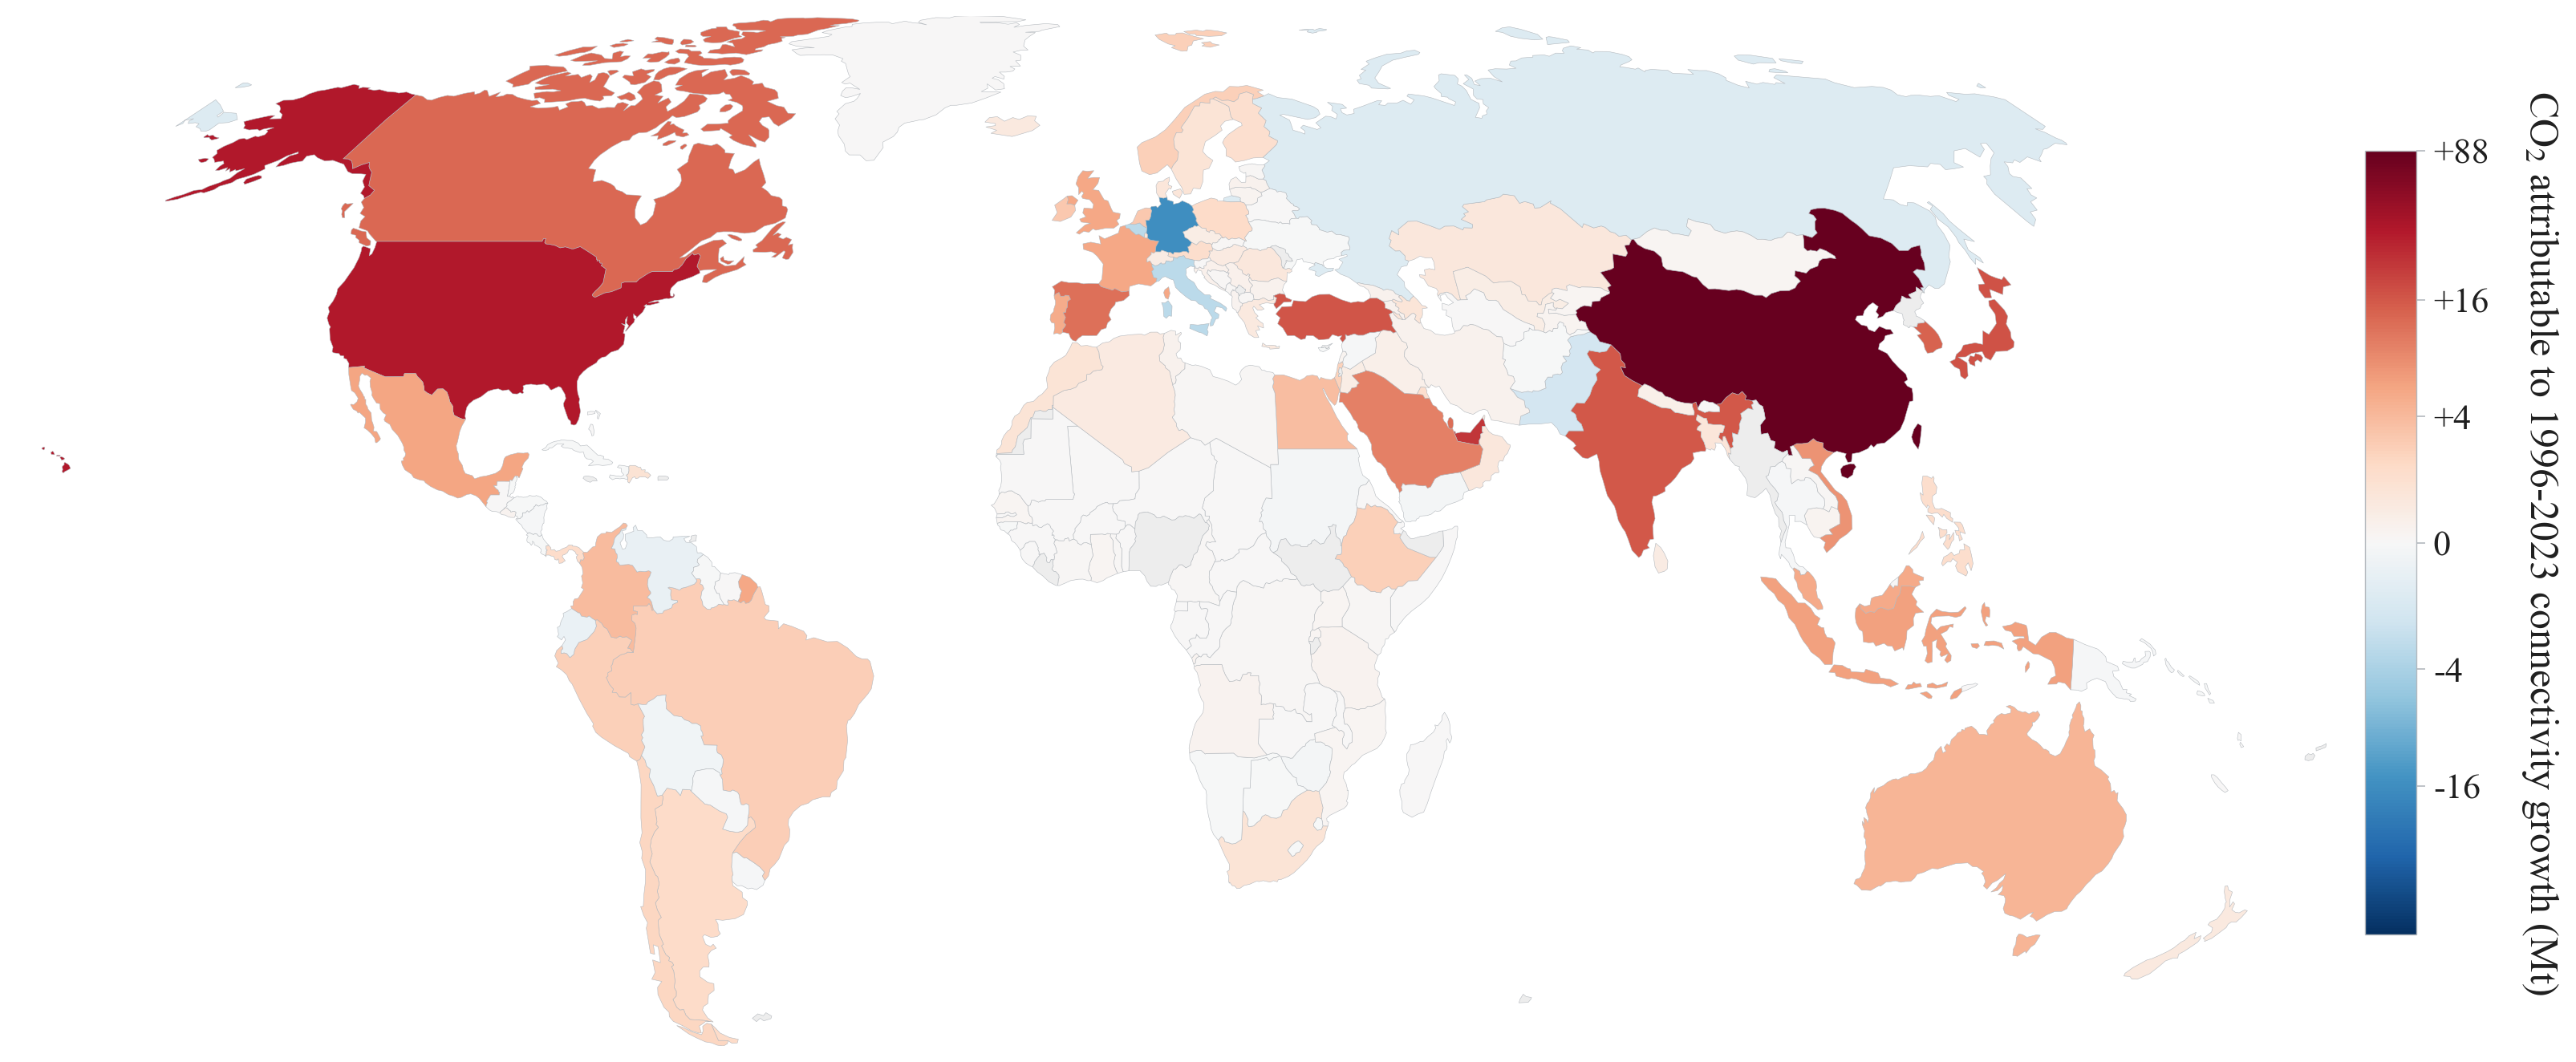
\includegraphics[width=0.92\textwidth]{CO2_map_attributed_2023.png}
\caption{\textbf{Aviation CO$_2$ attributed to post-1996 connectivity growth, 2023 (Mt).} White denotes zero; the attribution applies the Feyrer-instrument elasticity to each country's connectivity change.}
\label{fig:attributed}
\end{figure}

\begin{table}[htbp]
\centering
\begin{threeparttable}
\caption{Country-level attribution and social cost of connectivity-driven aviation CO$_2$, 2023}
\label{tab:scc}
\footnotesize
\begin{tabular}{lcccccc}
\toprule
 & & \multicolumn{2}{c}{Attributed CO$_2$ (Mt)} & \multicolumn{3}{c}{Social cost (\$bn per year)} \\
\cmidrule(lr){3-4}\cmidrule(lr){5-7}
 & $\Delta \ln$ GACI & Total & International & SCC \$51 & SCC \$185 & SCC \$190 \\
\midrule
China          & 0.33  & 87.7  & 16.9  & 4.5  & 16.2 & 16.7 \\
United States  & 0.04  & 36.4  & 13.6  & 1.9  & 6.7  & 6.9  \\
United Arab Emirates & 0.57 & 24.7 & 24.7 & 1.3 & 4.6 & 4.7 \\
Japan          & 0.19  & 17.4  & 10.4  & 0.9  & 3.2  & 3.3  \\
Turkey         & 0.55  & 16.6  & 13.5  & 0.8  & 3.1  & 3.2  \\
India          & 0.19  & 15.9  & 7.6   & 0.8  & 2.9  & 3.0  \\
Korea          & 0.71  & 14.1  & 12.8  & 0.7  & 2.6  & 2.7  \\
Canada         & 0.22  & 13.1  & 8.5   & 0.7  & 2.4  & 2.5  \\
Qatar          & 0.80  & 12.2  & 12.2  & 0.6  & 2.3  & 2.3  \\
Spain          & 0.14  & 11.8  & 9.5   & 0.6  & 2.2  & 2.3  \\
Germany        & $-0.09$ & $-15.8$ & $-15.2$ & $-0.8$ & $-2.9$ & $-3.0$ \\
\midrule
World          &       & 356.4 & 212.0 & 18.2 & 65.9 & 67.7 \\
\bottomrule
\end{tabular}
\begin{tablenotes}[flushleft]
\footnotesize
\item Notes: Attributed CO$_2$ applies the Feyrer-instrument elasticities (5.669 total, 5.690 international) to each country's 1996--2023 change in log connectivity: attributed share $= 1-\exp(-\beta\,\Delta\ln\mathrm{GACI}_c)$, applied to 2023 emission levels under the bunker convention. Social cost values one year's attributable emissions at three social-cost-of-carbon estimates (2020 USD per tonne of CO$_2$): the US Interagency Working Group interim value (\$51, 3 percent discount rate), Rennert et al.\ (2022) (\$185, 2 percent near-term discount rate), and the US EPA (2023) central value (\$190, 2 percent Ramsey discounting); the valuation recurs annually while the traffic persists. Top ten positive countries, Germany (largest negative), and the world total (184 countries); the world attributed total equals 42.5 percent of 2023 aviation CO$_2$. Because the elasticity exceeds one, country-level attributed shares are extreme for fast growers; the figures are partial-equilibrium accounting.
\end{tablenotes}
\end{threeparttable}
\end{table}

\begin{figure}[htbp]
\centering
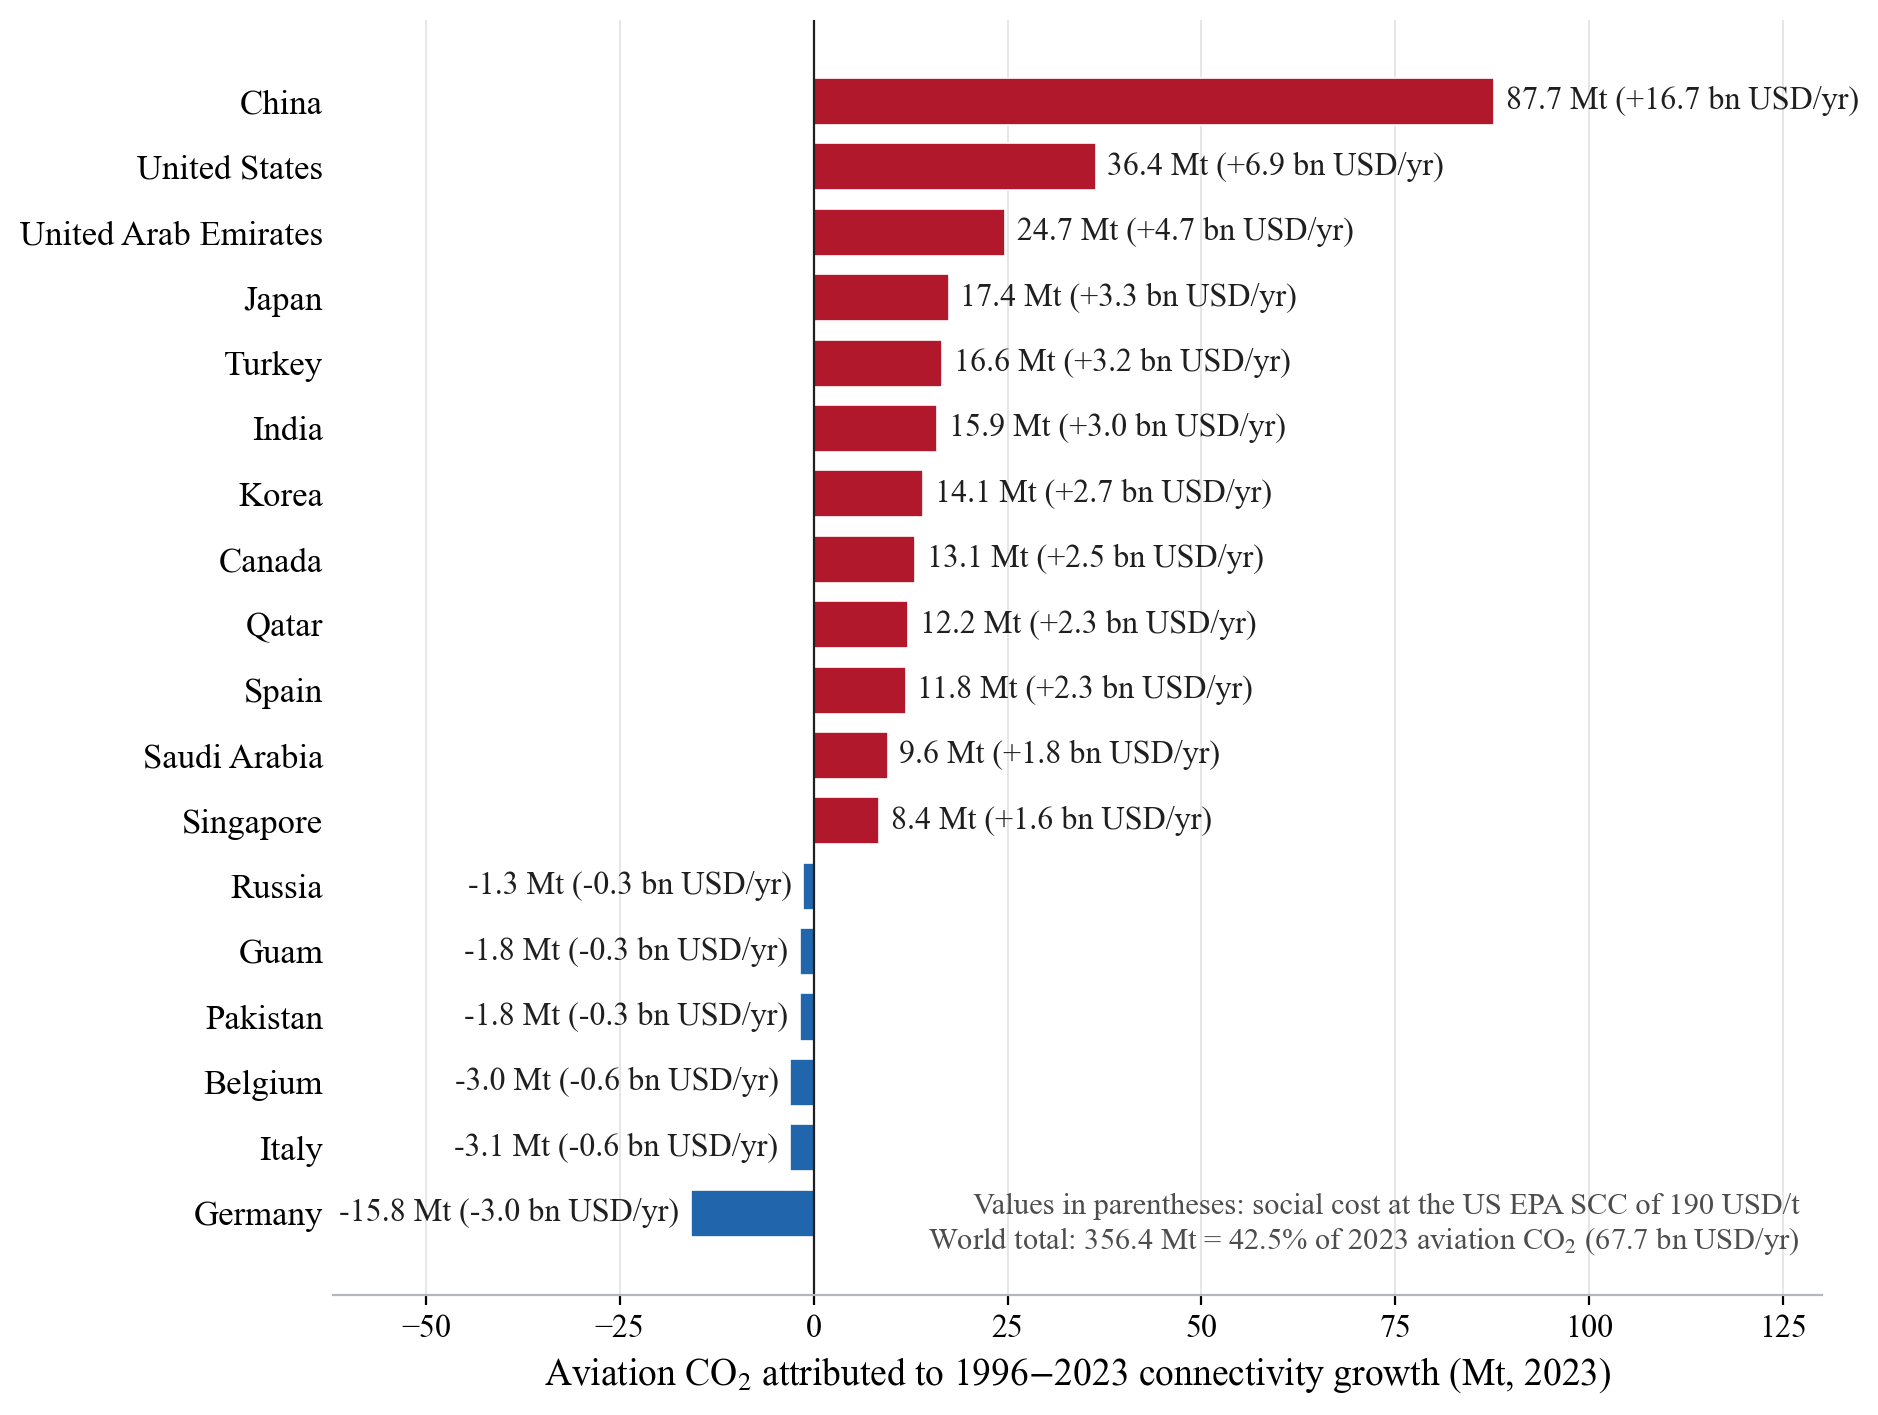
\includegraphics[width=0.92\textwidth]{CO2_attribution_bars.png}
\caption{\textbf{Country-level aviation CO$_2$ attributed to 1996--2023
connectivity growth, with its social cost.} Top twelve positive countries
and all countries below $-1$ Mt; parenthetical values apply the US EPA
social cost of carbon (\$190 per tonne). The world total is 356.4 Mt, 42.5
percent of 2023 aviation CO$_2$ (\$67.7 billion per year).}
\label{fig:bars}
\end{figure}

\begin{figure}[htbp]
\centering
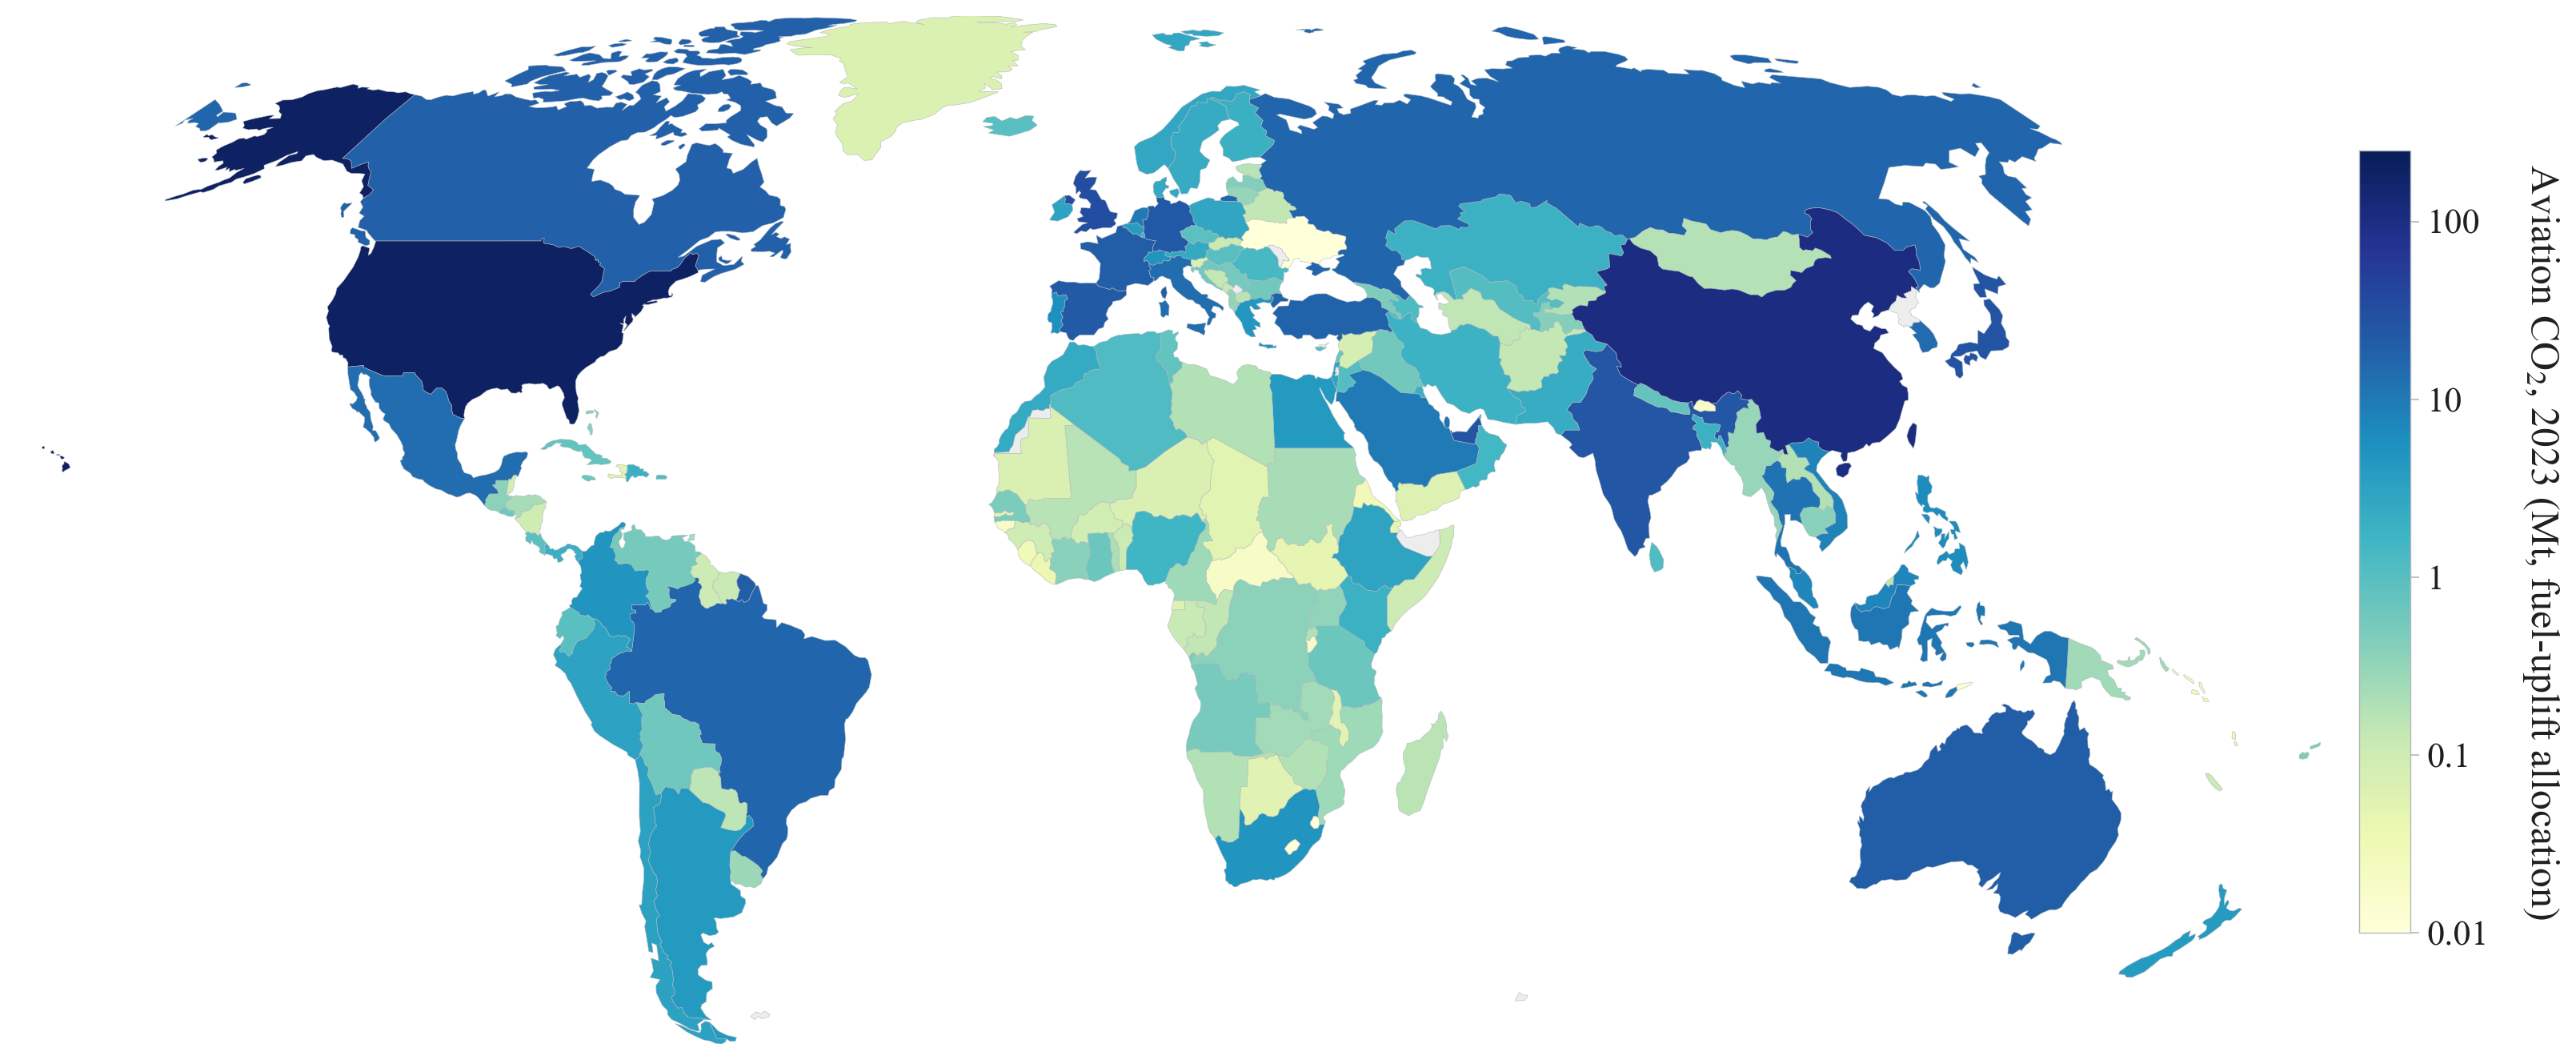
\includegraphics[width=0.92\textwidth]{CO2_map_levels_2023.png}
\caption{\textbf{Aviation CO$_2$ levels under the bunker convention, 2023.}}
\label{fig:levels}
\end{figure}

\begin{figure}[htbp]
\centering
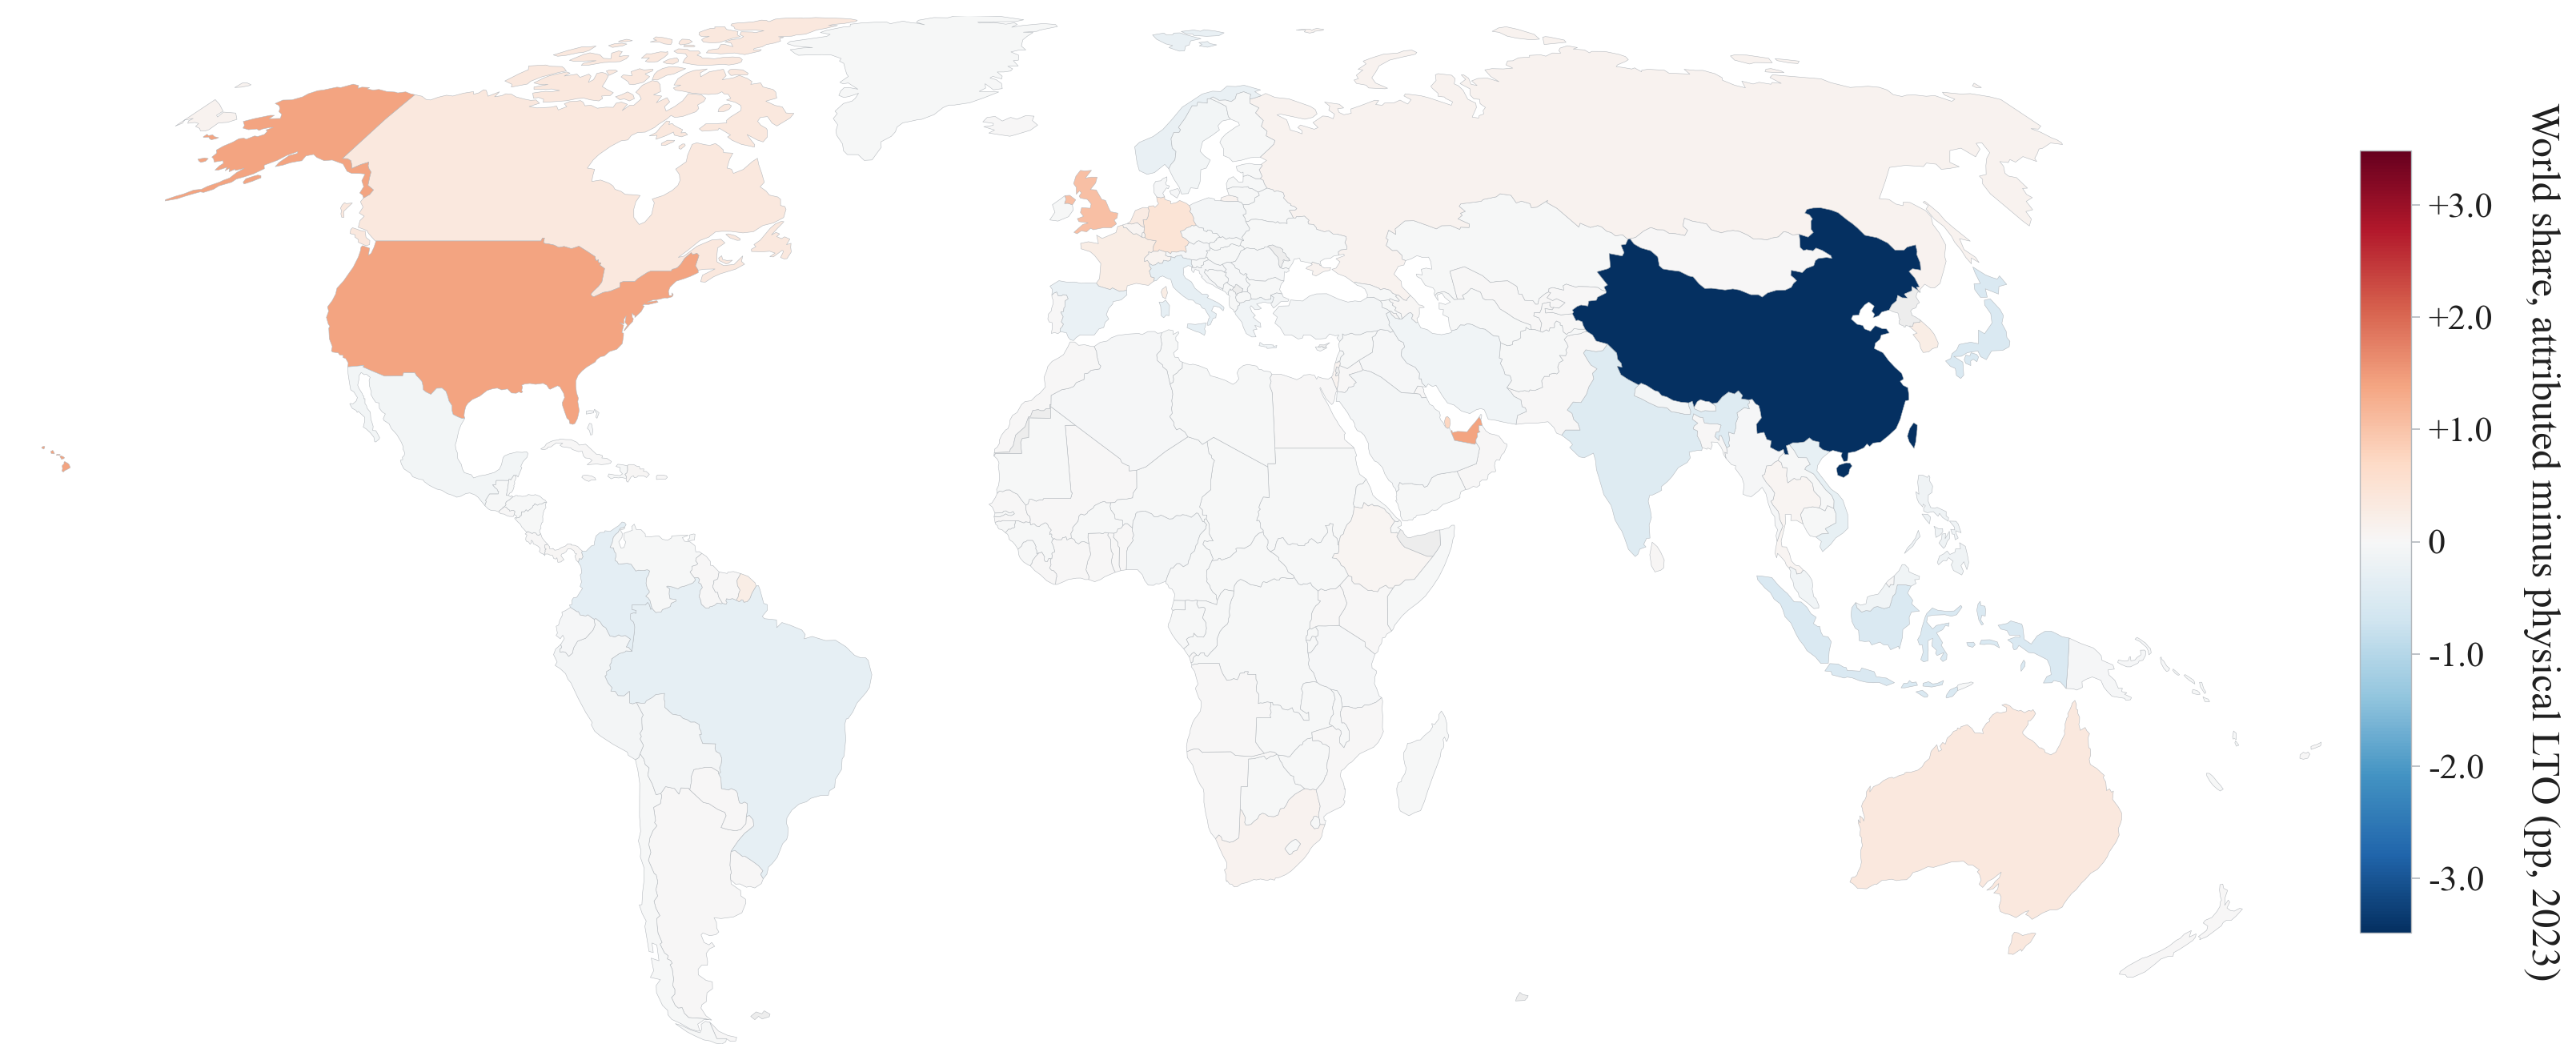
\includegraphics[width=0.92\textwidth]{CO2_map_mismatch_2023.png}
\caption{\textbf{Attribution mismatch, 2023:} bunker-attributed share minus physical LTO share (percentage points). Positive values indicate international hub countries; negative values indicate domestically oriented networks.}
\label{fig:mismatch}
\end{figure}

\subsection*{Only fuel switching materially lowers the level}
Since the efficiency margin does not offset the scale margin, the level of
emissions can be materially lowered only by changing the fuel burned.
Backing fuel quantities out of the 2023 total of 838 Mt and applying
ReFuelEU-style blending paths, the 2035 mandate lowers the total to
704--754 Mt and the 2050 mandate to 369--545 Mt, depending on the
life-cycle saving of sustainable aviation fuel (Fig.~\ref{fig:saf};
Methods). The full 2050 blending path with a life-cycle saving of at least
65 percent would offset emissions of the same magnitude as those attributed
to the connectivity growth of the past generation.

\begin{figure}[htbp]
\centering
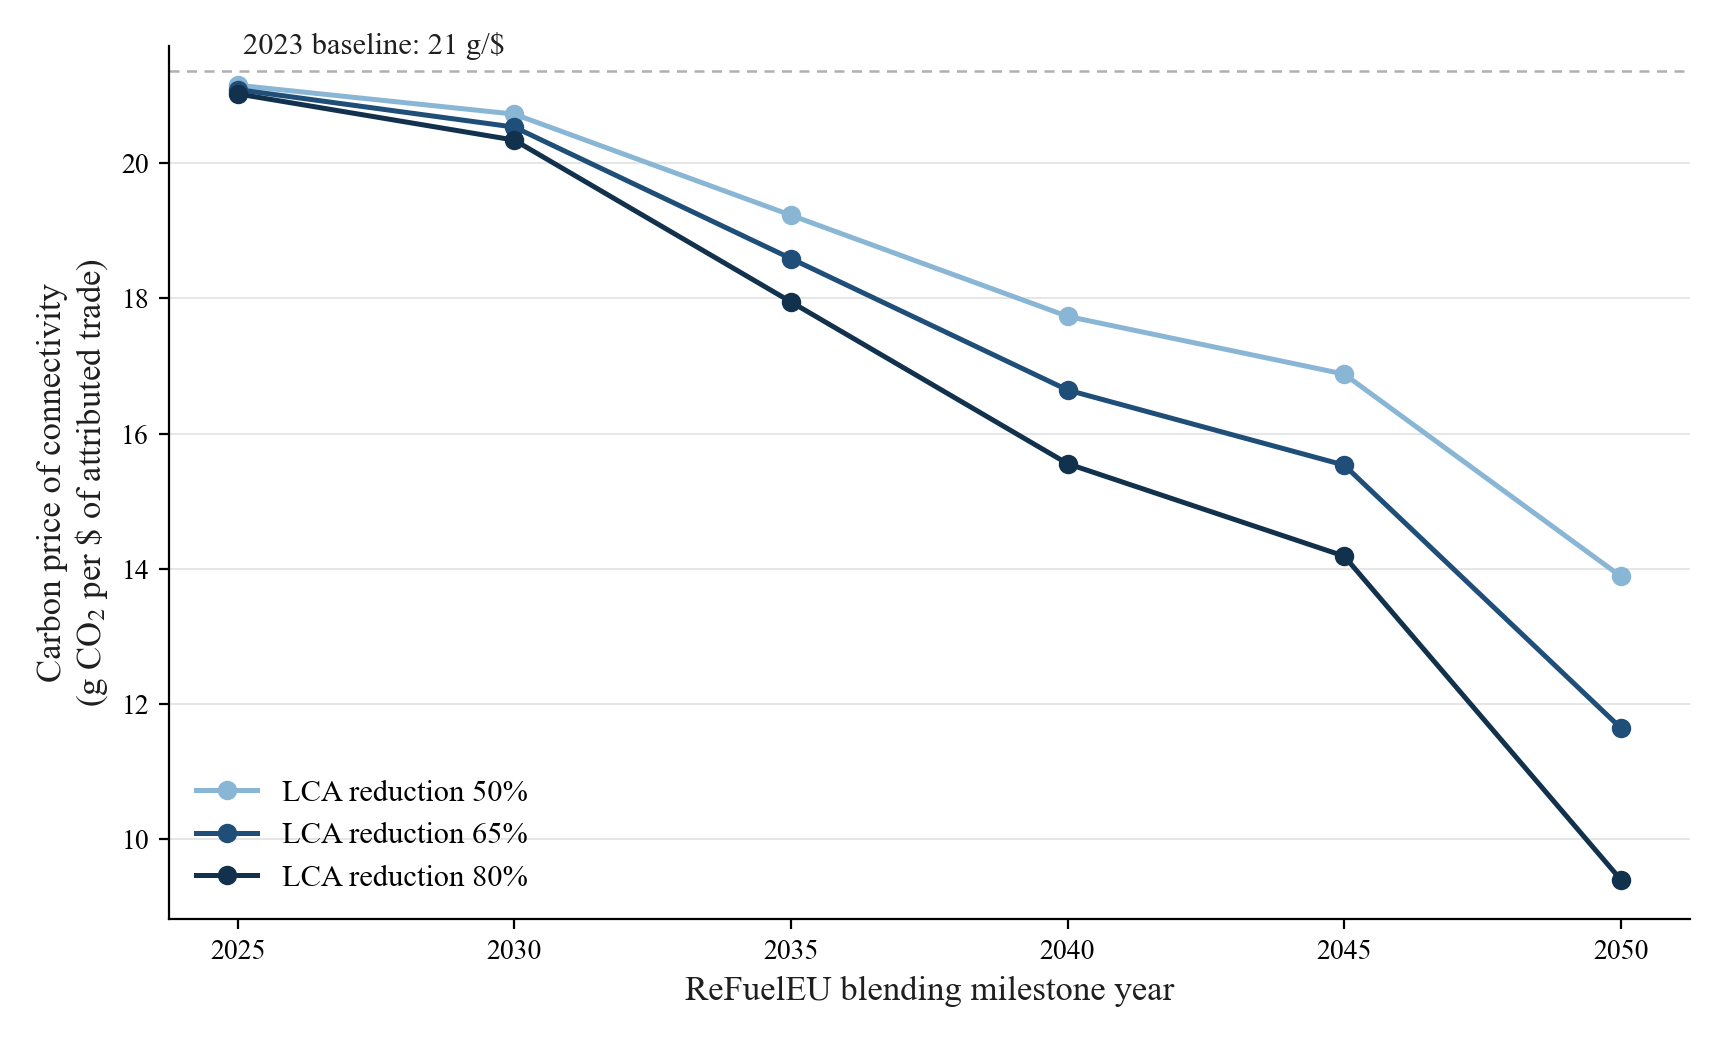
\includegraphics[width=0.92\textwidth]{CO2_saf_scenarios.png}
\caption{\textbf{World aviation CO$_2$ under ReFuelEU-style SAF blending paths.}}
\label{fig:saf}
\end{figure}

\subsection*{Attribution and fuel-switching scenarios [Ray and Lisa]}
The share of 2023 emissions attributed to post-1996 connectivity growth is
$1 - \exp(-\beta\,\Delta \ln \mathrm{GACI}_c)$, applied to 2023 levels;
because $\beta$ far exceeds one, country-level shares are extreme for
fast-growing countries and the world total (42.5 percent) is the more
conservative summary. Fuel-switching scenarios back fuel out of emissions
at 3.15 kg CO$_2$ per kg and apply ReFuelEU-style blending shares (2 to 70
percent over 2025--2050) with life-cycle savings of 50, 65, and 80 percent,
holding 2023 traffic fixed; the calculations are partial-equilibrium
accounting. Attributed emissions are monetised at three
social-cost-of-carbon estimates, in 2020 USD per tonne of CO$_2$: the US
Interagency Working Group interim value (\$51, 3 percent discount rate),
the estimate of Rennert et al.\ (2022) (\$185, 2 percent near-term
discount rate), and the US EPA (2023) central value (\$190, 2 percent
Ramsey discounting) [TODO cite]. The valuation applies to one year's
attributable emissions and recurs annually while the connectivity-driven
traffic persists.

%=======================================================================
\section*{Discussion [Jinwoo]}
%=======================================================================
Three implications follow. First, for climate policy, the efficiency gains
that accompany network development are not a decarbonisation strategy. The
technique margin is present at both the country and airport levels, but it
offsets less than one tenth of the scale response, and only sustained fuel
switching materially lowers the emissions level. Policies that promote
connectivity on economic grounds should be evaluated jointly with fuel and
demand-side instruments rather than on the expectation that hub efficiency
will absorb the growth in traffic.

Second, for the geography of mitigation burden, the results identify two
distinct wedges. The spillover estimates show that a country's emissions
respond to its neighbours' connectivity, so national accounting misses a
regional externality. The attribution analysis shows in addition that
accounting conventions reallocate measured responsibility across countries
by up to 3.5 percentage points of the world total. Both wedges bear
directly on instruments, such as CORSIA, that assign obligations on the
basis of booked emissions.

Third, several limitations qualify the estimates. Emissions are
schedule-based and do not reflect load factors, so they measure the carbon
content of scheduled capacity. The primary instrument is strongest in the
network-expansion era, and the later-period elasticity is identified only
when the COVID-19 collapse years are excluded. No causal estimate is
available at the airport level. The
attribution and fuel-switching calculations are partial-equilibrium
accounting exercises, and non-CO$_2$ climate effects of aviation are
outside the scope of this study.

%=======================================================================
\section*{Methods}
%=======================================================================
\subsection*{Emissions data [Chunan and Fangyu]}
We compute flight-level CO$_2$ from OAG schedules under the EEA/EMEP
Guidebook (2023) framework (Section 1.A.3.a): fuel burn by engine type and
stage length, multiplied by a fixed emission factor (3.15 kg CO$_2$ per kg
Jet~A; 3.10 for AvGas). The data are stage-resolved at the airport-month
level, separately for domestic and international traffic, on the departure
side (taxi-out, take-off, climb-out, cruise) and the arrival side
(approach, taxi-in, cruise), together with flights, seats, and
seat-kilometres. Coverage is 1996 through the first half of 2024; the
partial month of July 2024 is dropped and the annual analysis ends in 2023.
Emissions are schedule-based, so they reflect scheduled capacity rather
than realised load factors [FANGYU: check description].

\subsection*{Allocation rules[Chunan and Fangyu]}
Because the stages are recorded separately, national emissions can be
constructed under three conventions without double counting: a territorial
rule using landing-and-take-off (LTO) emissions only; a fuel-uplift
(bunker) rule assigning cruise emissions to the departure country, our
headline measure; and a 50/50 split of cruise emissions between endpoint
countries. Cruise is recorded once per flight side and used once.

\subsection*{Validation [Chunan and Fangyu]}
The 2019 world total is 0.919 Gt against the ICCT estimate of 0.92 Gt; the
LTO share is 11.8 percent; the log-log correlation with the OWID/ICCT
country series is 0.99 in all overlapping years, with a level ratio of
1.05--1.10 consistent with full-capacity scheduling. The match to the
connectivity panel is complete at the airport-year level after crosswalk
corrections.

\subsection*{GACI [Chunan and Fangyu]}
Connectivity is the GACI panel (constructed following Cheung et al.\ 2020)
for 1996--2024, aggregated to the country level as the capacity-weighted
mean of airport scores, with the maximum, unweighted mean, and sum as
alternatives. The estimation sample covers 184 countries over 1996--2023,
$N = 4{,}634$.

\subsection*{Estimation [Junya]}
The estimating equation is
\begin{equation}
\ln \mathrm{CO_2}_{ct} = \beta \,\ln \mathrm{GACI}_{ct}
 + \gamma \,\ln \mathrm{pop}_{ct} + \delta \,\ln \mathrm{seaMA}_{ct}
 + \alpha_c + \tau_t + \varepsilon_{ct},
\label{eq:main}
\end{equation}
estimated by two-stage least squares with country and year fixed effects
and robust standard errors.

\subsection*{Instruments and validity [Junya]}
Connectivity is instrumented with a Feyrer-type shifter that interacts
world aviation technology $a_t$ with the country's air market access
computed on fixed 1996 geography, while the sea-distance market-access
channel is controlled directly. The identifying variation is the
differential exposure of countries to the global growth of aviation implied
by their geography, holding the surface-shipping alternative fixed; the
first-stage Kleibergen--Paap $F$ is 154. Because any shifter of the form
(global cycle $\times$ baseline characteristic) may proxy (global cycle
$\times$ country size), we re-estimate each first stage adding interactions
of the global cycle with baseline population, GDP, and airport capacity.
The primary instrument survives ($F$ declines only from 120.1 to 105.8);
a tourism-heritage instrument does not (13.8 to below 1) and is used only
as a lens on the composition margin, its compliers being hub-quality
changes with a post-2010 first stage; an airport-level heritage-proximity
pilot fails the same test (59.5 to 2.3) and was abandoned, so airport-level
results are descriptive. Plausibly-exogenous bounds indicate that a direct
effect of the instrument would need to account for 85 percent of the
reduced form (42 percent for intensity) to overturn the results; quintile
reduced forms are reported in Extended Data Fig.~\ref{fig:rfquintile}.

\subsection*{Spillover design [Junya]}
Neighbour connectivity is the inverse-distance-weighted average of all
other countries' log GACI, with weights based on haversine distances
between countries' aviation activity centroids, and is instrumented by the
identically weighted average of their Feyrer shifters. The own shifter
enters directly, so the own-connectivity effect is estimated in reduced
form; own and neighbour connectivity cannot be jointly instrumented because
the two shifters are nearly collinear within country.

\subsection*{Mediation [Junya]}
The instrumental-variable decomposition instruments the treatment with the
Feyrer shifter in both the mediator and outcome equations and combines the
paths by the product method with delta-method standard errors; the Imai,
Keele and Yamamoto algorithm is implemented by quasi-Bayesian simulation on
least-squares models with country and year indicators. Each mediator is
analysed separately and the mediators overlap, so shares do not sum.



\subsection*{Data availability}
[TODO: OAG licensing statement; GACI panel availability; replication
archive.]

\subsection*{Code availability}
[TODO: replication code archive.]

%=======================================================================
% Extended Data (ED Tables 1-3, ED Figures 1-6)
% At submission these move to the Extended Data template; numbering below
% is by order of citation in the main text.
%=======================================================================
\clearpage
\section*{Extended Data}

\begin{table}[htbp]
\centering
\begin{threeparttable}
\caption{Extended Data Table 1: Temporal split of the connectivity elasticity}
\label{tab:temporal}
\footnotesize
\begin{tabular}{lcccc}
\toprule
 & \multicolumn{1}{c}{Bunker CO$_2$} & \multicolumn{1}{c}{Intl.\ CO$_2$} & \multicolumn{1}{c}{Seat-km} & \multicolumn{1}{c}{Intensity} \\
 & (1) & (2) & (3) & (4) \\
\midrule
\multicolumn{5}{l}{\textit{Panel A. Full sample, 1996--2023}} \\
  ln GACI (cwm) & 5.669$^{***}$ & 5.690$^{***}$ & 6.068$^{***}$ & -0.399$^{***}$ \\
   & (0.412) & (0.415) & (0.443) & (0.118) \\
  KP $F$ & 153.6 & 152.7 & 153.6 & 153.6 \\
  $N$ & 4,634 & 4,633 & 4,634 & 4,634 \\
\midrule
\multicolumn{5}{l}{\textit{Panel B. Network-expansion era, 1996--2007}} \\
  ln GACI (cwm) & 5.613$^{***}$ & 5.809$^{***}$ & 4.837$^{***}$ & 0.776$^{***}$ \\
   & (0.665) & (0.704) & (0.626) & (0.249) \\
  KP $F$ & 75.0 & 74.9 & 75.0 & 75.0 \\
  $N$ & 1,883 & 1,882 & 1,883 & 1,883 \\
\midrule
\multicolumn{5}{l}{\textit{Panel C. Mature-network era, 2010--2023 (excl.\ 2020--2021)}} \\
  ln GACI (cwm) & 3.005$^{***}$ & 2.965$^{***}$ & 3.984$^{***}$ & -0.979$^{***}$ \\
   & (0.635) & (0.610) & (0.668) & (0.248) \\
  KP $F$ & 36.7 & 36.7 & 36.7 & 36.7 \\
  $N$ & 2,065 & 2,065 & 2,065 & 2,065 \\
\midrule
\multicolumn{5}{l}{\textit{Panel D. Unrestricted split: 1996--2009}} \\
  ln GACI (cwm) & 6.109$^{***}$ & 6.262$^{***}$ & 5.537$^{***}$ & 0.571$^{***}$ \\
   & (0.565) & (0.590) & (0.534) & (0.192) \\
  KP $F$ & 127.7 & 126.9 & 127.7 & 127.7 \\
  $N$ & 2,218 & 2,217 & 2,218 & 2,218 \\
\midrule
\multicolumn{5}{l}{\textit{Panel E. Unrestricted split: 2010--2023 (weak first stage)}} \\
  ln GACI (cwm) & 1.213 & 1.051 & 1.829 & -0.617 \\
   & (1.394) & (1.463) & (1.598) & (0.739) \\
  KP $F$ & 7.0 & 7.0 & 7.0 & 7.0 \\
  $N$ & 2,415 & 2,415 & 2,415 & 2,415 \\
\bottomrule
\end{tabular}
\begin{tablenotes}[flushleft]
\footnotesize
\item Notes: 2SLS with the Feyrer instrument; specifications as in Table~\ref{tab:main}. Panels B and C split the sample at its midpoint (2010) and exclude the crisis years: Panel B ends before the global financial crisis (2008--2009) and Panel C drops the COVID-19 collapse (2020--2021). Both subperiods are strongly identified and the elasticity in each is above one; the pre-versus-post difference for total CO$_2$ is 2.61 ($p = 0.005$). Panels D and E report the unrestricted split for reference: the weak first stage in Panel E (KP $F = 7.0$) is driven by the COVID years, whose exclusion in Panel C restores $F$ to 36.7, so the small point estimates in Panel E reflect a contaminated first stage rather than a vanished effect. Robust standard errors in parentheses. $^{***}$, $^{**}$, $^{*}$: significance at 1, 5, and 10 percent.
\end{tablenotes}
\end{threeparttable}
\end{table}

\begin{table}[htbp]
\centering
\begin{threeparttable}
\caption{Extended Data Table 2: Heterogeneity of the connectivity elasticity}
\label{tab:hetero}
\footnotesize
\begin{tabular}{lcccc}
\toprule
 & Coefficient & s.e. & KP $F$ & $N$ \\
\midrule
\multicolumn{5}{l}{\textit{Panel A. Total CO$_2$ by baseline income tercile}} \\
  Low income & 11.431$^{***}$ & (1.338) & 35.2 & 1,595 \\
  Middle income & 5.906$^{***}$ & (0.782) & 48.2 & 1,547 \\
  High income & 0.350 & (1.106) & 10.1 & 1,491 \\
\midrule
\multicolumn{5}{l}{\textit{Panel B. Total CO$_2$ by baseline connectivity tercile}} \\
  Low connectivity & 9.018$^{***}$ & (0.656) & 117.4 & 1,452 \\
  Middle connectivity & 5.642$^{***}$ & (0.908) & 29.9 & 1,526 \\
  High connectivity & 0.452 & (2.201) & 1.8 & 1,655 \\
\midrule
\multicolumn{5}{l}{\textit{Panel C. Total CO$_2$ by region}} \\
  Europe & 0.236 & (0.616) & 55.5 & 1,189 \\
  Asia--Pacific & 5.424$^{***}$ & (0.667) & 64.4 & 1,110 \\
  Africa & 8.385$^{***}$ & (1.688) & 20.2 & 1,230 \\
  Latin America & 3.229$^{***}$ & (0.900) & 14.1 & 683 \\
  Middle East & \multicolumn{4}{c}{not identified (KP $F<2$)} \\
  North America & \multicolumn{4}{c}{not identified (KP $F<2$)} \\
\midrule
\multicolumn{5}{l}{\textit{Panel D. Intensity by baseline income tercile}} \\
  Low income & -1.057$^{***}$ & (0.299) & 35.5 & 1,596 \\
  Middle income & -0.372 & (0.241) & 48.2 & 1,547 \\
  High income & 1.012 & (0.715) & 10.1 & 1,491 \\
\bottomrule
\end{tabular}
\begin{tablenotes}[flushleft]
\footnotesize
\item Notes: Split-sample 2SLS with the Feyrer instrument; terciles are formed on 1996 values. All specifications include country and year fixed effects and control for log population and log sea market access. The Middle East and North America cells have too little instrument variation for inference. Robust standard errors in parentheses. $^{***}$, $^{**}$, $^{*}$: significance at 1, 5, and 10 percent.
\end{tablenotes}
\end{threeparttable}
\end{table}

\begin{table}[htbp]
\centering
\begin{threeparttable}
\caption{Extended Data Table 3: Causal mediation of the connectivity effect on aviation CO$_2$}
\label{tab:mediation}
\footnotesize
\begin{tabular}{lccccc}
\toprule
\multicolumn{6}{l}{\textit{Panel A. Instrumental-variable product of coefficients (2SLS scale; total effect 5.669)}} \\
Mediator & $a$: GACI$\rightarrow M$ & $b$: $M\rightarrow$CO$_2$ & ACME ($a\times b$) & Sobel $p$ & Share mediated \\
\midrule
  Flight frequency & 6.976 & 0.682 & 4.756 & 0.000 & 83.9\% \\
  Seat-kilometres & 6.068 & 0.808 & 4.901 & 0.000 & 86.5\% \\
  International share & 0.096 & -1.060 & -0.102 & 0.060 & -1.8\% \\
\midrule
\multicolumn{6}{l}{\textit{Panel B. Imai, Keele and Yamamoto (2010) mediation (OLS scale; total effect 3.582)}} \\
Mediator & ACME & Direct effect & Total effect & & Share mediated \\
\midrule
  Flight frequency & 1.766 & 1.816 & 3.582 & & 49.3\% \\
  Seat-kilometres & 3.424 & 0.159 & 3.583 & & 95.6\% \\
  International share & -0.077 & 3.657 & 3.580 & & -2.1\% \\
\bottomrule
\end{tabular}
\begin{tablenotes}[flushleft]
\footnotesize
\item Notes: Outcome is log total bunker CO$_2$; the treatment is log GACI (capacity-weighted mean). Panel A instruments the treatment with the Feyrer shifter in each equation and combines the paths by the product method with delta-method (Sobel) standard errors. Panel B implements the algorithm of Imai, Keele and Yamamoto (2010) by quasi-Bayesian simulation (200 draws) on least-squares models with country and year indicator variables. Each row is a separate single-mediator analysis and the mediators overlap, so shares do not sum across rows. All models control for log population and log sea market access. Sequential ignorability of the mediator is assumed conditional on the fixed effects.
\end{tablenotes}
\end{threeparttable}
\end{table}


\begin{figure}[htbp]
\centering
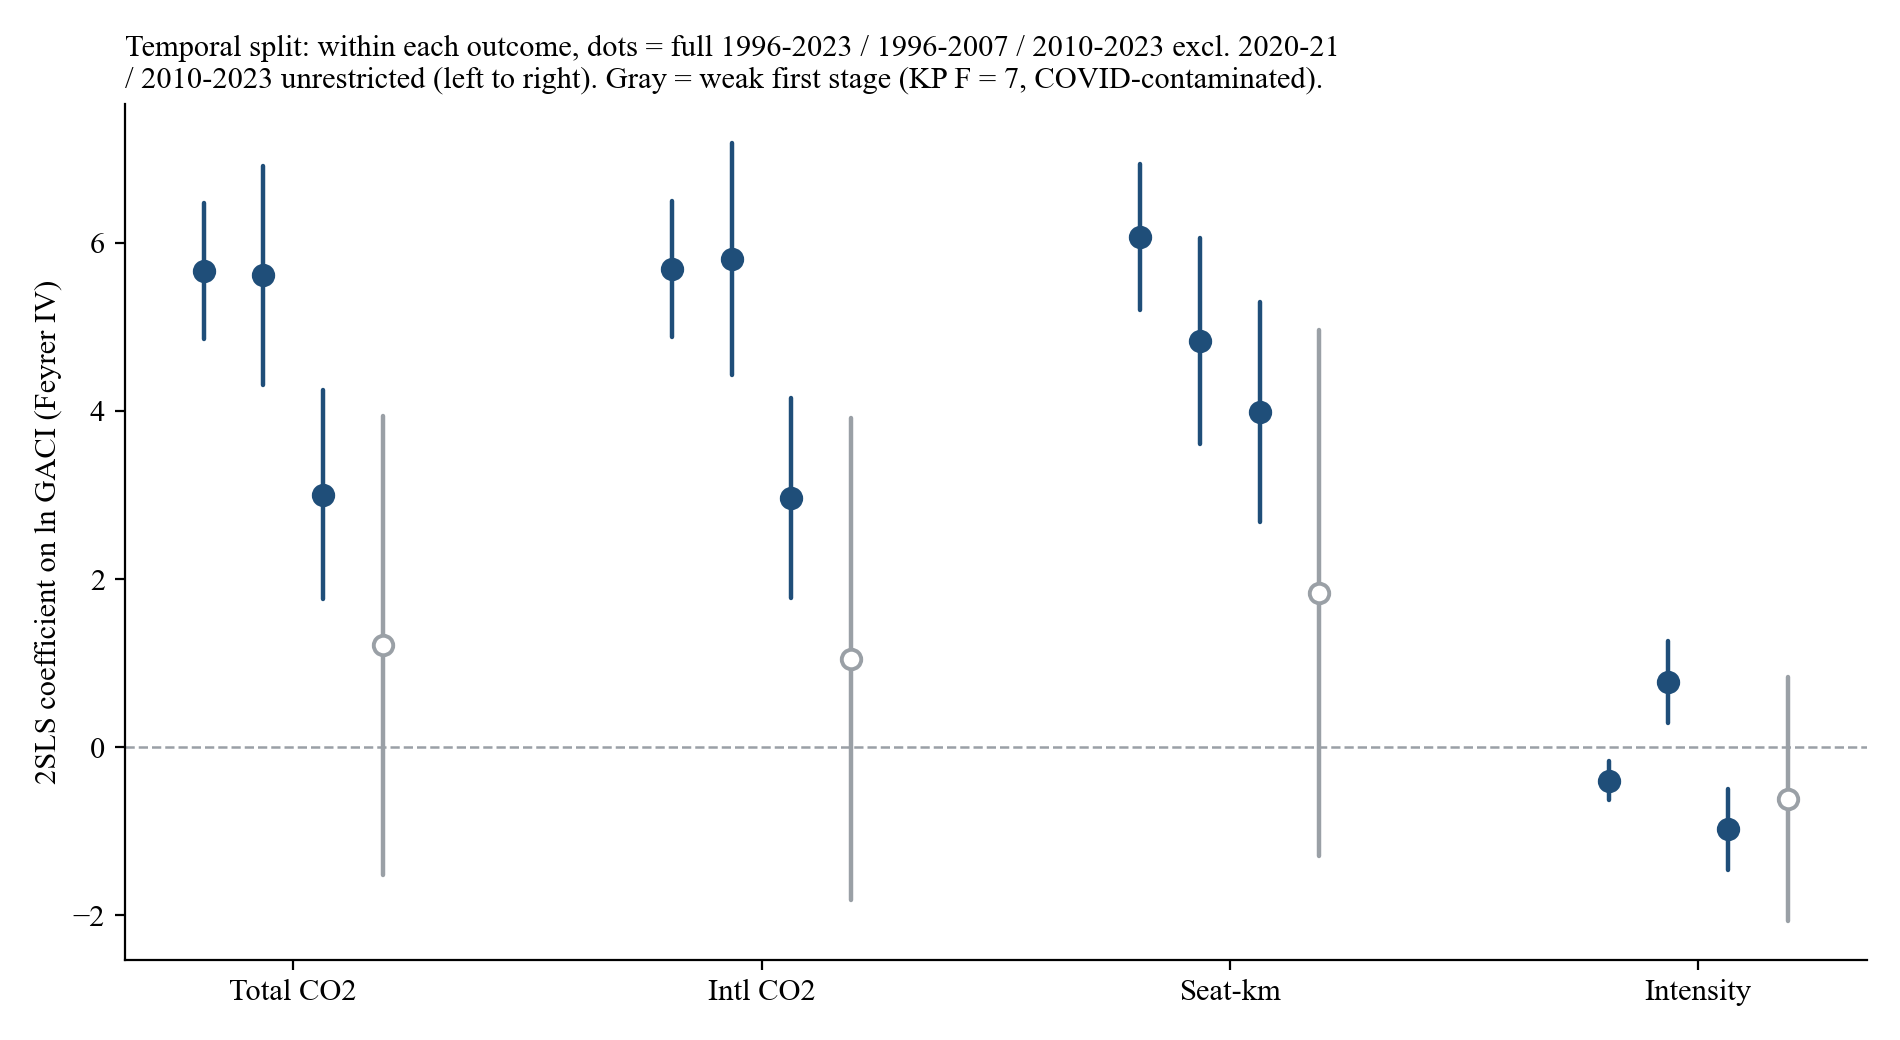
\includegraphics[width=0.92\textwidth]{CO2_temporal_coefplot.png}
\caption{Extended Data Fig.\ 1: Temporal split of the connectivity elasticity. Within each outcome, markers show the full sample, the network-expansion era (1996--2007), the mature-network era (2010--2023 excluding the COVID-19 years 2020--2021), and the unrestricted 2010--2023 sample from left to right; gray denotes the unrestricted later sample, whose first stage (KP $F=7$) is contaminated by the COVID collapse.}
\label{fig:temporal}
\end{figure}

\begin{figure}[htbp]
\centering
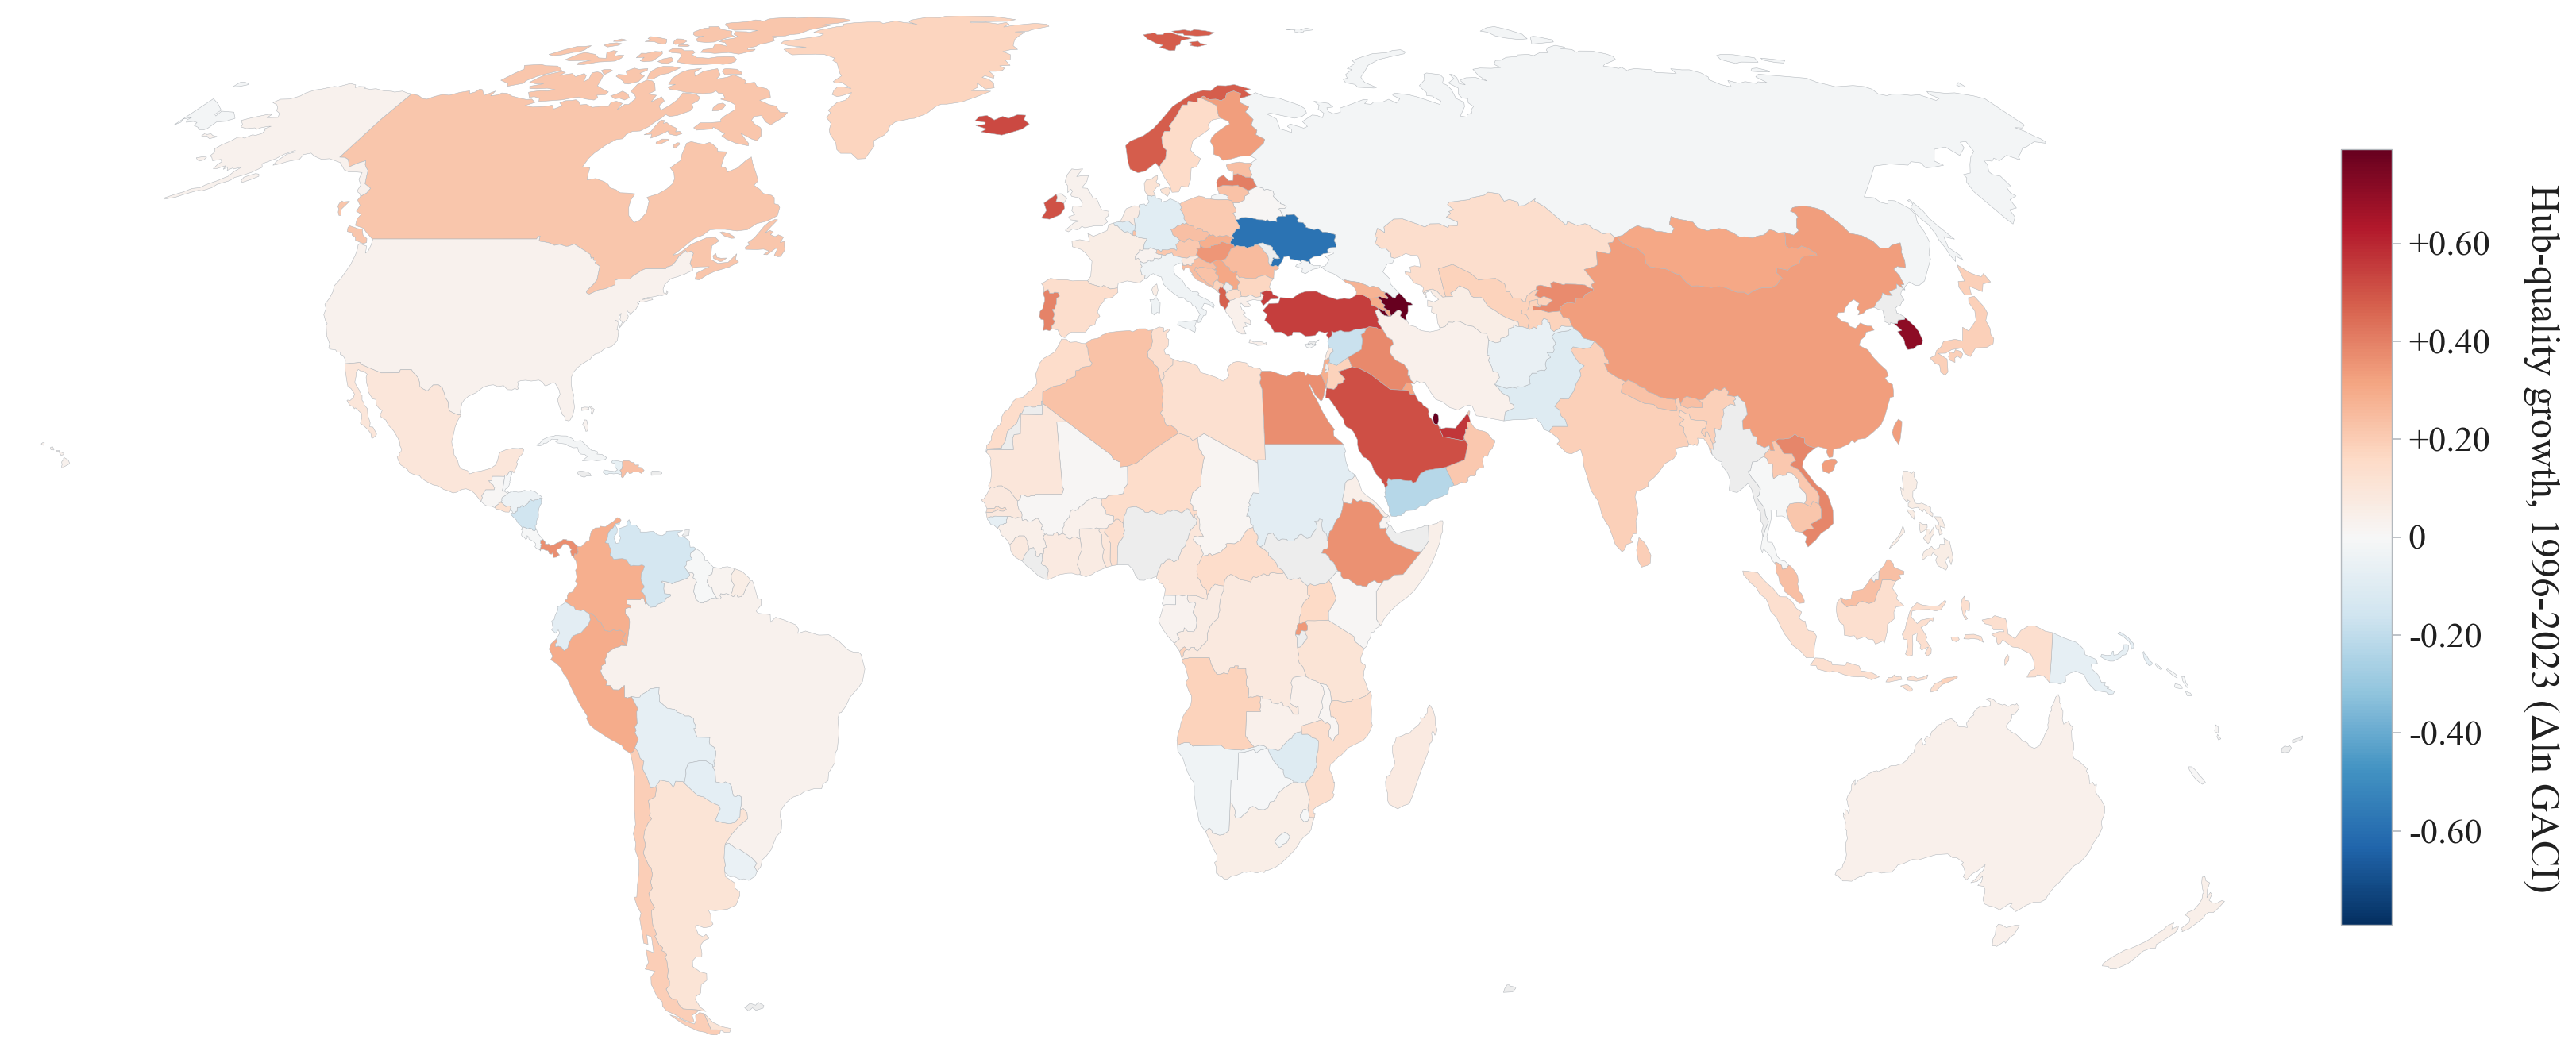
\includegraphics[width=0.92\textwidth]{CO2_map_dlngaci.png}
\caption{Extended Data Fig.\ 2: Change in log air connectivity (GACI, capacity-weighted mean), 1996--2023.}
\label{fig:dlngaci}
\end{figure}



\begin{figure}[htbp]
\centering
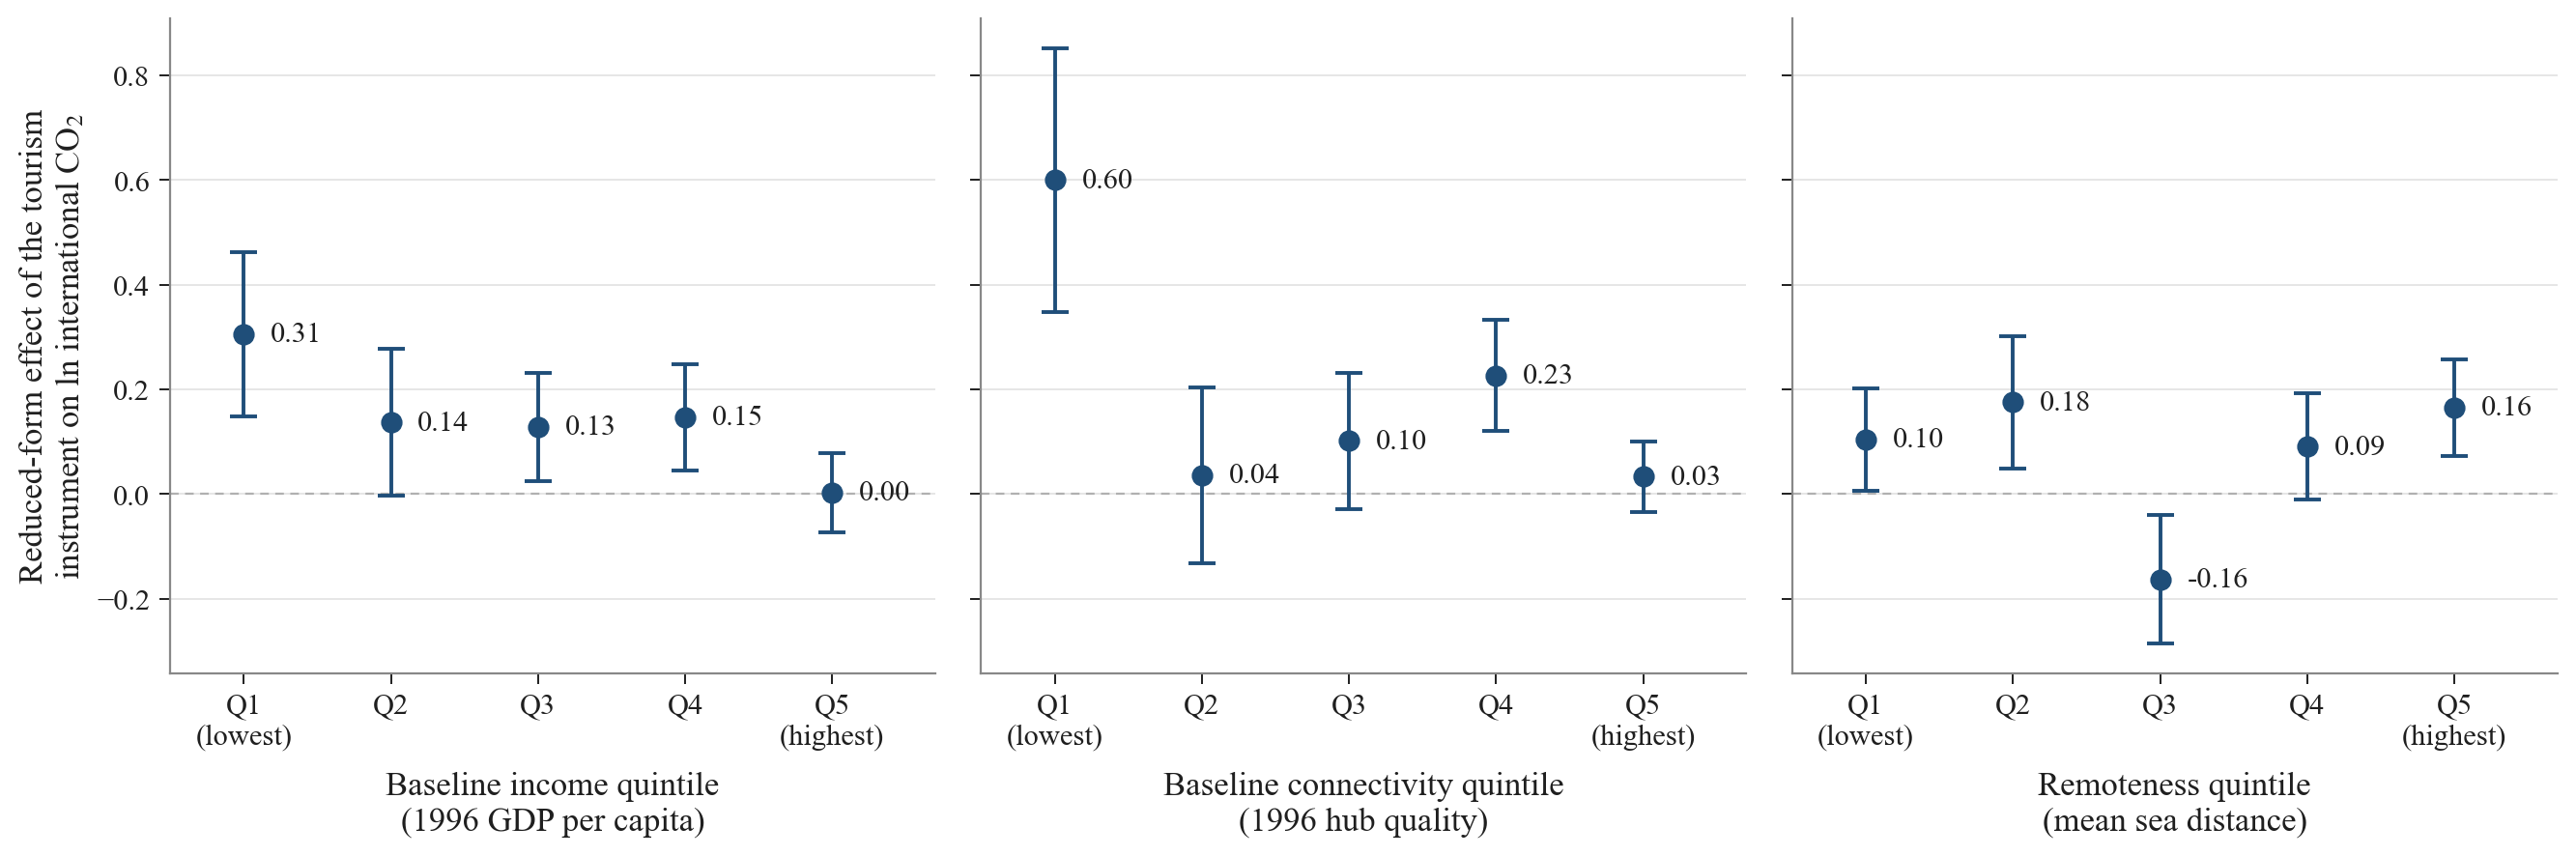
\includegraphics[width=0.92\textwidth]{CO2_rf_quintile.png}
\caption{Extended Data Fig.\ 3: Reduced-form quintile slopes under the tourism shifter: effects are concentrated in low-income, low-connectivity quintiles.}
\label{fig:rfquintile}
\end{figure}

% Carbon-intensity-of-trade-gains map retained from the heritage pipeline
% (v1 framing, dropped from the main text per Sunbin; kept pending a
% decision).
\begin{figure}[htbp]
\centering
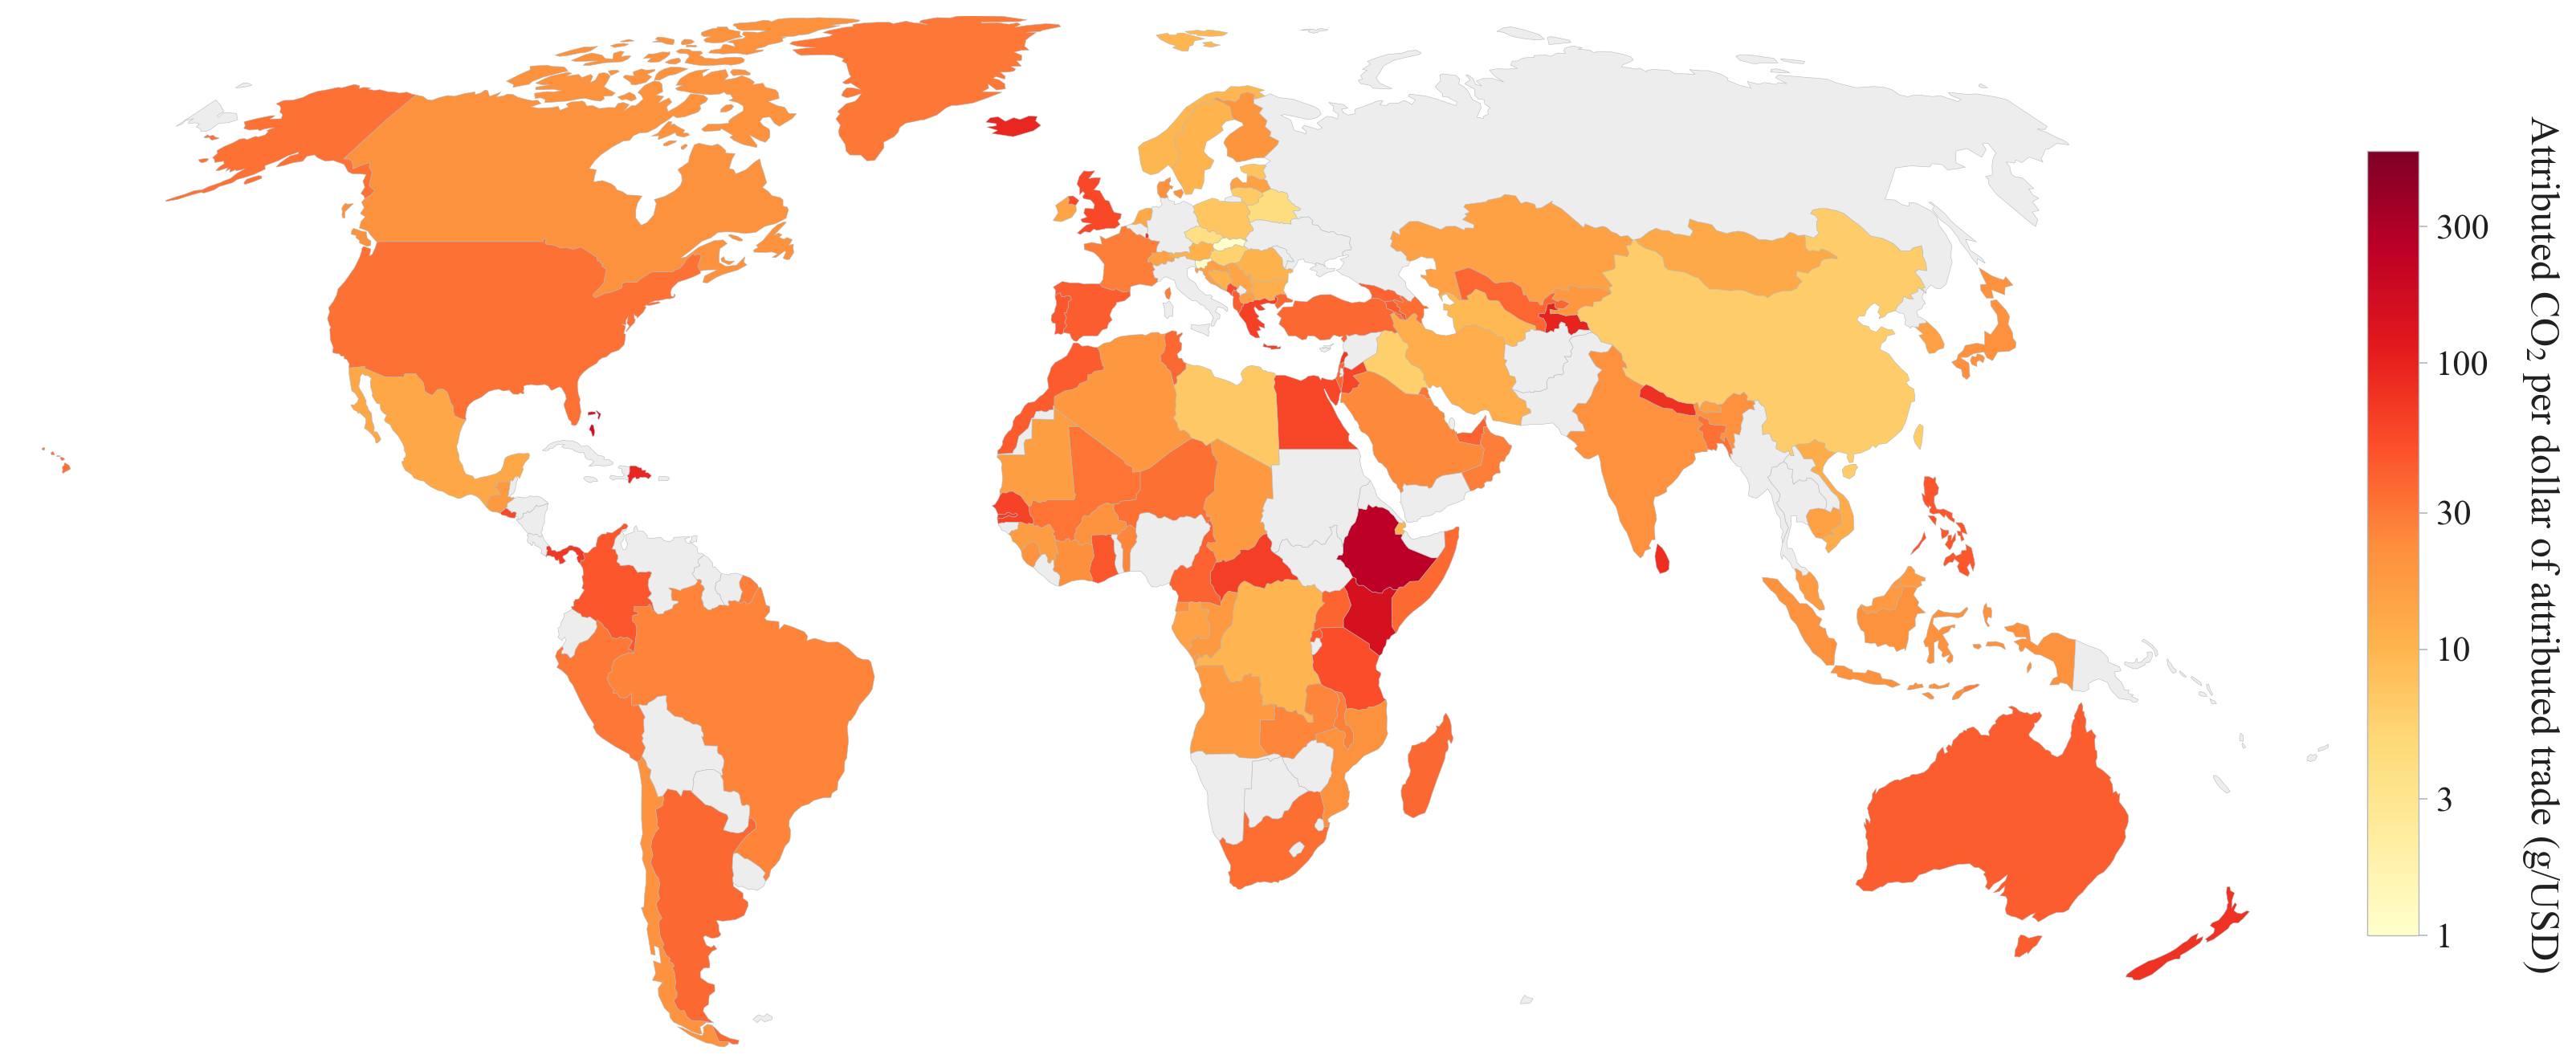
\includegraphics[width=0.92\textwidth]{CO2_map_carbonprice.png}
\caption{Extended Data Fig.\ 4: Carbon intensity of connectivity gains (g CO$_2$ per USD of trade gain; heritage-instrument pipeline).}
\label{fig:carbonprice}
\end{figure}

\end{document}
